% Time-stamp: <2022-11-08 07:39:29 A13258Q>
% Amine Raboun 2023, https://amineraboun.github.io/
% Romain Lafarguette 2023, https://romainlafarguette.github.io/

%% ---------------------------------------------------------------------------
%% Preamble: Packages and Setup
%% ---------------------------------------------------------------------------
% Class 
\documentclass{beamer}

% Theme
\usetheme{Boadilla}
\usecolortheme{dolphin}
%\setbeamertemplate{headline}{} % Remove the top navigation bar

% Font and encoding
\usepackage[utf8]{inputenc} % Input font
\usepackage[T1]{fontenc} % Output font
\usepackage{lmodern} % Standard LateX font
\usefonttheme{serif} % Standard LateX font

% Maths 
\usepackage{amsfonts, amsmath, mathabx, bm, bbm} % Maths Fonts

% Graphics
\usepackage{graphicx} % Insert graphics
\usepackage{subfig} % Multiple figures in one graphic
\graphicspath{{/../static/img}{/../static/diagrams}}



% Layout
\usepackage{changepage}

% Colors
\usepackage{xcolor}
\definecolor{imfblue}{RGB}{0,76,151} % Official IMF color
\setbeamercolor{title}{fg=imfblue}
\setbeamercolor{frametitle}{fg=imfblue}
\setbeamercolor{structure}{fg=imfblue}

% Tables
\usepackage{booktabs,rotating,multirow} % Tabular rules and other macros
%\usepackage{pdflscape,afterpage} % Landscape mode and afterpage
%\usepackage{threeparttable} % Split long tables
\usepackage[font=scriptsize,labelfont=scriptsize,labelfont={color=imfblue}]{caption}

% Import files
\usepackage{import}

% Appendix slides
\usepackage{appendixnumberbeamer} % Manage page numbers for appendix slides

% References
\usepackage{hyperref}
\usepackage{blkarray}
\usepackage{amsmath}

% A few macros: environments
\newenvironment{wideitemize}{\itemize\addtolength{\itemsep}{10pt}}{\enditemize}
\newenvironment{wideenumerate}{\enumerate\addtolength{\itemsep}{10pt}}{\endenumerate}

\newenvironment{extrawideitemize}{\itemize\addtolength{\itemsep}{30pt}}{\enditemize}
\newenvironment{extrawideenumerate}{\enumerate\addtolength{\itemsep}{30pt}}{\endenumerate}

% Remove navigation symbols and other superfluous elements
\setbeamertemplate{navigation symbols}{}
\beamertemplatenavigationsymbolsempty

%\setbeamertemplate{note page}[plain]
\hypersetup{pdfpagemode=UseNone} % don't show bookmarks on initial view
\setbeameroption{hide notes}

% Institute font
\setbeamerfont{institute}{size=\footnotesize}
\DeclareMathSizes{10}{9}{7}{5}  

%% ---------------------------------------------------------------------------
%% Title info
%% ---------------------------------------------------------------------------
\title[Time series Econometrics]{Time series Econometrics (Theory}
\author[R. Lafarguette, A. Raboun]{Romain Lafarguette, Ph.D. Amine Raboun, Ph.D.}
\institute[IMF STX]{Quant \& IMF External Expert\thanks{\scriptsize{\emph{This training material is the property of the International Monetary Fund (IMF) and is intended for use in IMF courses. Any reuse requires the permission of the IMF.}}} \\
\begin{center}
{\href{https://romainlafarguette.github.io/}{\textcolor{imfblue}{https://romainlafarguette.github.io/}}} \end{center}
\begin{center}
{\href{https://amineraboun.github.io/}{\textcolor{imfblue}{https://amineraboun.github.io/}}} \end{center}
} 

\date[STI, 17 April 2023]{Singapore Training Institute, 17 April 2023}

\titlegraphic{\vspace{-0.75cm}
    \begin{figure}
    \centering
    \subfloat{{
\includegraphics[width=2cm]{../static/img/imf_logo}}}%
    \end{figure}}


% Slide between sections
\AtBeginSection[]
{
    \begin{frame}
        \frametitle{Table of Contents}
        \tableofcontents[currentsection]
    \end{frame}
}

%% ---------------------------------------------------------------------------
%% Title slide
%% ---------------------------------------------------------------------------
\begin{document}

\begin{frame}
\maketitle
\end{frame}



\section{Statistical Features and Properties}

\begin{frame}
  \frametitle{Stylized Properties}

  Fan and Yao (2015, the Elements of Financial Econometrics) identify 8 main "stylized facts"
  
  \begin{enumerate}
  \item Stationarity
  \item Absence of autocorrelations
  \item Heavy tails
  \item Asymmetry
  \item Volatility clustering
  \item Aggregational Gaussianity
  \item Long range dependence
  \item Leverage effect
  \end{enumerate}
  
\end{frame}



\begin{frame}
  \frametitle{Stationarity}
  \begin{exampleblock}{Example}
   In general, prices are non-stationary but returns are stationary 
 \end{exampleblock}

 \begin{block}{Definition: Weak Stationarity (Second Order Stationarity)}
   A stochastic process ${X_t}_{t \in \mathbb{Z}}$ is weakly stationary if and only if:

   \begin{itemize}
   \item $\mathbb{E}(X^2_t) \ < \ \infty \ \quad \forall \ t \ \in \ \mathbb{Z}$
   \item $\mathbb{E}(X_t) = \mu \ \quad \forall \ t \ \in \ \mathbb{Z}$ doesn't depend on $t$
   \item $\text{Cov}(x_t, x_{t+h}) \ = \ \mathbb{E}[(x_{t+h} - m)(x_t - m)] \ = \ \gamma_h \quad \forall \ (t, h) \ \in \ \mathbb{Z}^2$ desn't depend on $t$
   \end{itemize}
   
 \end{block}
 
\end{frame}


\begin{frame}
  \frametitle{Intuitive Interpretation}
   Weak stationarity means that the stochastic process oscillates around a constant level, is not trended and has the following properties:\\
  
  \begin{wideenumerate}
  \item The mean and time-covariance are constant over time
    \begin{equation*}
\mathbb{E}(X_t) = \mu \qquad \mathbb{C}ov(X_t, X_{t-h}) = \gamma(h) \qquad \forall \ h \ \in \ \mathbb{Z}
\end{equation*}
\item Because the time-covariance is constant over time, it implies that the variance is also constant over time
  \begin{equation*}
\mathbb{V}(X_t) = \mathbb{C}ov(X_t, X_{t-h}) = \gamma(0) \qquad \forall \ t \ \in \ \mathbb{Z}
  \end{equation*}
\item $\mathbb{C}ov(X_t, X_{t-h}) = \gamma(h) \qquad \forall \ h \ \in \ \mathbb{Z}$ can be interpreted as "\emph{covariance doesn't change when shifted in time}"
  \begin{equation*}
\mathbb{C}ov(X_r, X_s) = \mathbb{C}ov(X_{r+t}, X_{s+t}) \qquad \forall \ (r, s, t) \ \in \ \mathbb{Z}^3
  \end{equation*}
  
  \end{wideenumerate}
\end{frame}


\begin{frame}
\frametitle{Prices are Usually Non-Stationary...}
\makebox[\linewidth]{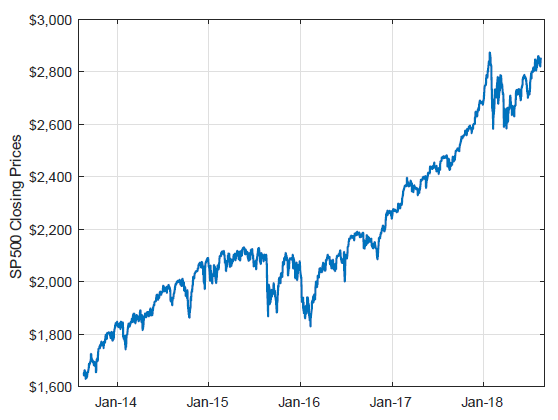
\includegraphics[width=0.7\paperwidth]{../static/course_1_img/non stationarity prices sp500.PNG}}
\hspace*{15pt}\hbox{\scriptsize Credit:\thinspace{\scriptsize\itshape Christophe Hurlin}}
\end{frame}


\begin{frame}
\frametitle{... But Returns Are !}
\makebox[\linewidth]{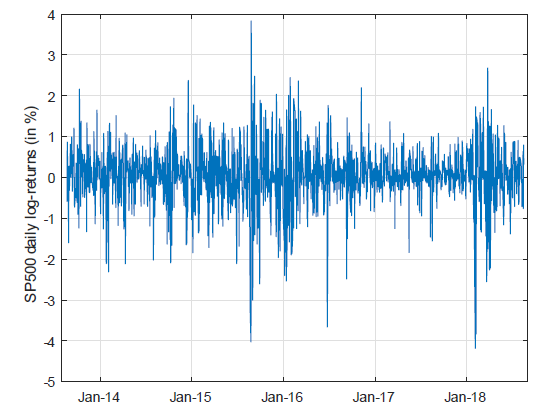
\includegraphics[width=0.7\paperwidth]{../static/course_1_img/stationarity returns sp500.PNG}}
\hspace*{15pt}\hbox{\scriptsize Credit:\thinspace{\scriptsize\itshape Christophe Hurlin}}
\end{frame}


\begin{frame}
  \frametitle{Absence of autocorrelations}
  \begin{exampleblock}{Fact: Common absence of autocorrelations}
    The autocorrelations of assets returns (in general) are often insignificant, except for very small intraday time scales (around 20 minutes) for which the microstructure effects come into play
  \end{exampleblock}

\textbf{Note:} The fact that returns hardly show any serial correlation does not mean that they are independent


\begin{block}{Definition: Autocorrelation}
  The autocorrelation, denoted $\rho(k)$ of a weak stationary process $X_t$ is the correlation between the values of the process at different times:

  \begin{equation*}
    \rho_k \ = \ \text{Corr}(X_t, X_{t-k}) \ = \ \frac{\mathbb{E}\left[ (X_t - \mu)(X_{t-k} - \mu)\right]}{\mathbb{V}(X_t)} = \frac{\gamma_k}{\sigma^2}
  \end{equation*}

with $\mu = \mathbb{E}[X_t]$, $\sigma^2 = \mathbb{V}(X_t), \ \forall \ t$ and $\gamma_k$ the autocovariance of order $k$
  
\end{block}

\end{frame}

\begin{frame}
  \frametitle{Measuring Sample Autocorrelation}
  \begin{block}{Definition: Sample Autocorrelation}
    The \textbf{sample autocorrelation}, denoted $\hat{\rho}(k)$ of a weak stationary process $X$ is an estimator of $\rho(k)$ defined as:

    \begin{equation*} 
      \hat{\rho}_k = \text{corr}(X_t, X_{t-k}) = \frac{1}{(T-k)\hat{\sigma^2}} \sum_{t=k+1}^{R}(X_t - \hat{\mu})(X_{t-k} - \hat{\mu})
    \end{equation*}
where $\hat{\sigma^2}$ and $\hat{\mu}$ are consistent estimators of $\mu = \mathbb{E}(X_t)$ and $\sigma^2 = \mathbb{V}(X_t) \qquad \forall t$
  \end{block}
\end{frame}



\begin{frame}
  \frametitle{Autocorrelation and Partial Autocorrelation}

  \begin{itemize}
  \item Autocorrelation: $\text{corr}(X_t, X_{t-k})$
  \item Partial Autocorrelation: $\text{corr}(X_t - \tilde{X}_{t}, \tilde{X}_t - \tilde{X}_{t-k})$ where $\tilde{X}_{j}$ is a linear combination of the stochastic process that minimize the MSE of $X_{j}$
  \item Intuition: the partial autocorrelation at lag k is the correlation after removing the effect of any correlations due to the terms at shorter lags
  \end{itemize}
  
  \makebox[\linewidth]{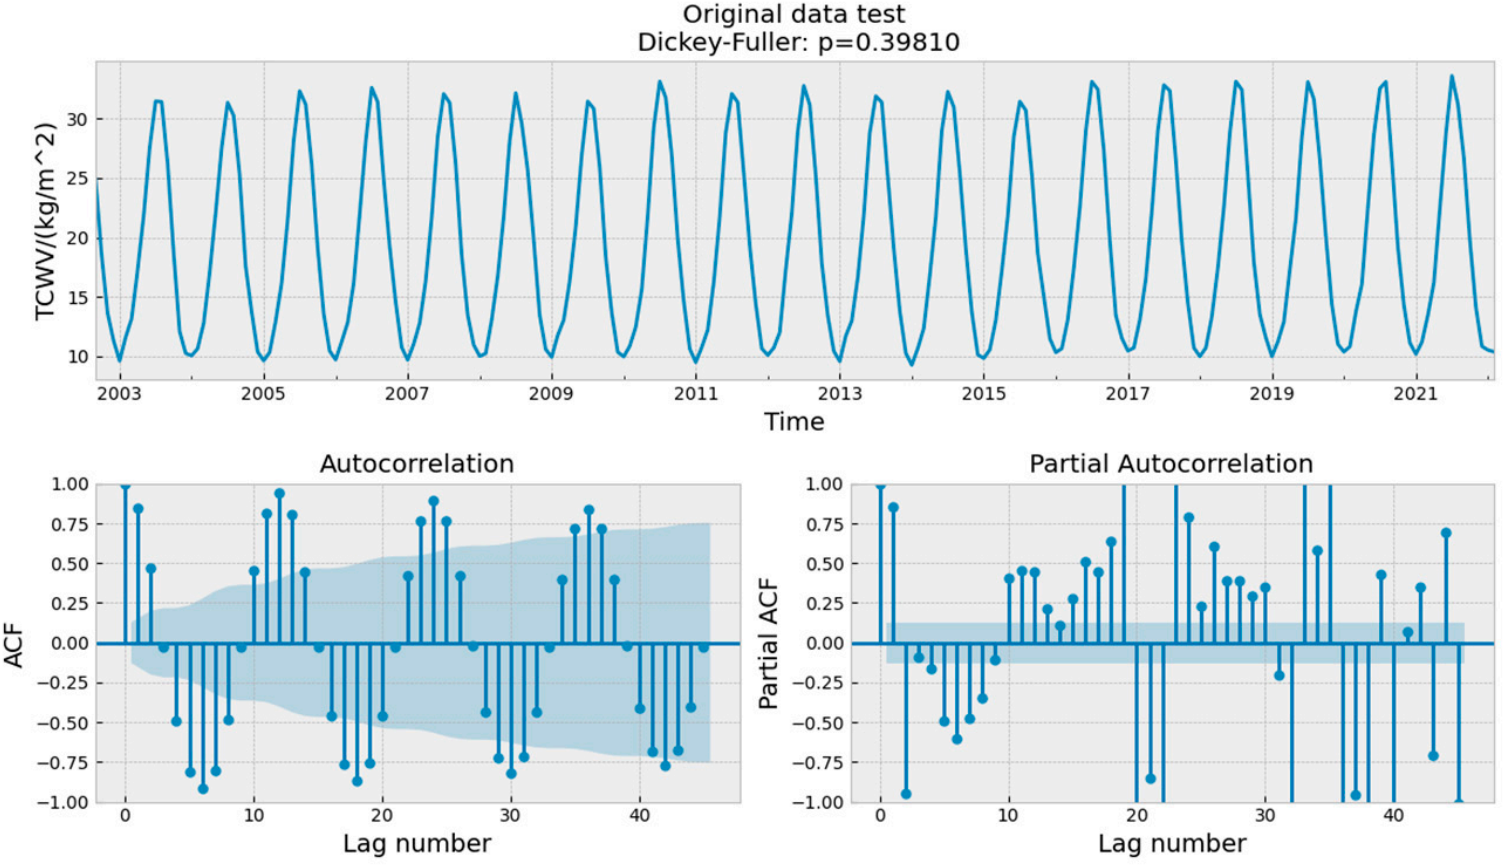
\includegraphics[width=0.6\paperwidth]{../static/course_1_img/acf_pacf.PNG}}
  \hspace*{15pt}\hbox{\scriptsize Credit:\thinspace{\scriptsize\itshape Shangguan, S et al. \emph{Atmosphere} (2022)}} 
\end{frame}

\begin{frame}
  \frametitle{Example: Autocorrelation of the SP500}
  The \textbf{Autocorrelation Function (ACF)} (or \textbf{correlogram}) represents the sample autocorrelation for different lags, from $k=1$ to a maximum lag order, for instance $k=15$

 \makebox[\linewidth]{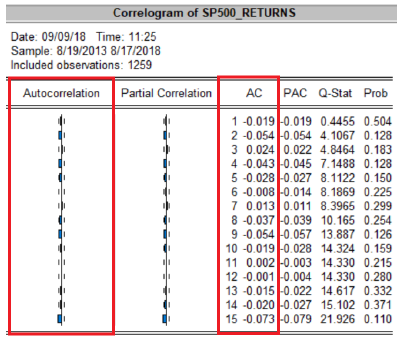
\includegraphics[width=0.5\paperwidth]{../static/course_1_img/autocorrelogram.PNG}}
 \hspace*{15pt}\hbox{\scriptsize Credit:\thinspace{\scriptsize\itshape Christophe Hurlin}} 
\end{frame}



\begin{frame}
  \frametitle{Asymmetry}

  \begin{block}{Stylized Fact: Heavy Tails}
    The distribution of many financial variables, including asset returns, are often \textbf{asymmetric} and \textbf{negatively skewed}
  \end{block}

  \begin{itemize}
  \item Asymmetry is defined by the skewness, which is the third-order moment (see before)
  \item This reflects the fact that the downturns of financial markets are often much steeper than the recoveries
  \item Investors tend to react more strongly to negative news that to positive news 
  \end{itemize}
\end{frame}


\begin{frame}
  \frametitle{Skewness}
  There are different shapes of kurtosis 
  \makebox[\linewidth]{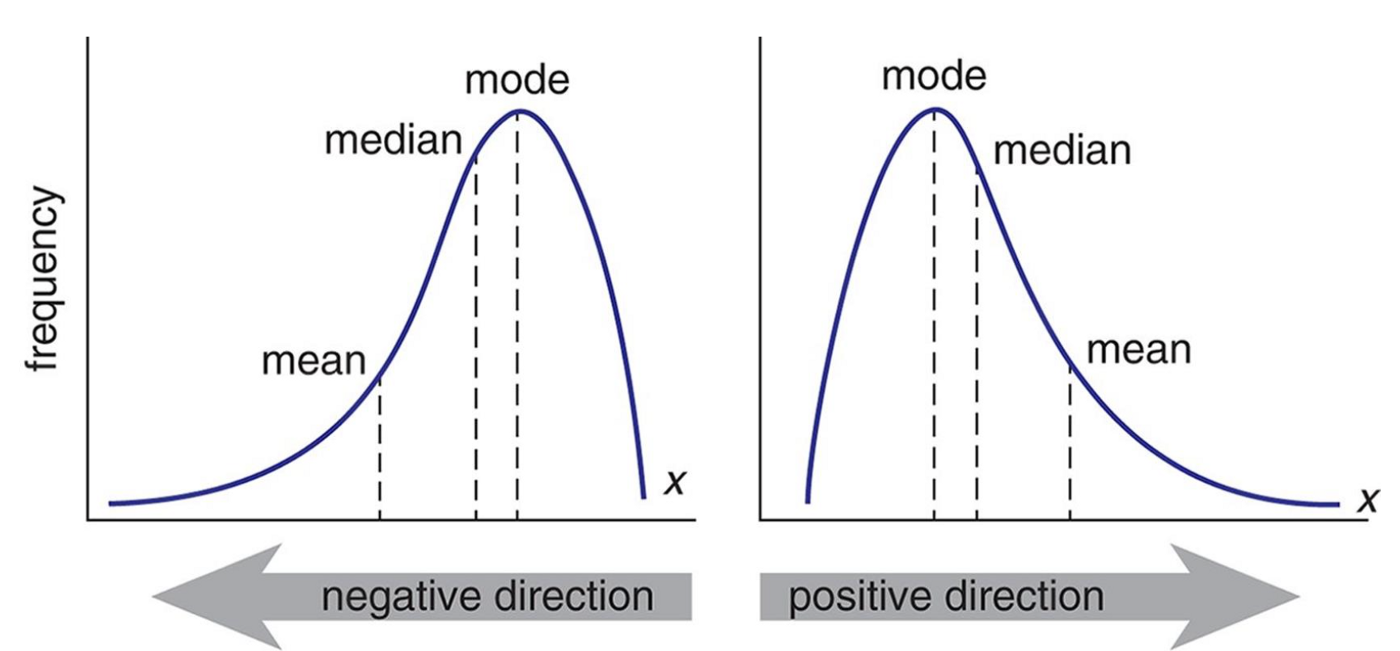
\includegraphics[width=0.8\paperwidth]{../static/course_1_img/skewness.PNG}}
  \hspace*{15pt}\hbox{\scriptsize Credit:\thinspace{\scriptsize\itshape Towards Data Science}} 
\end{frame}



\begin{frame}
  \frametitle{Heavy Tails}
  \begin{exampleblock}{Fact: Heavy Tails}
    The probability distribution of many financial variables, including asset returns, often exhibit \textbf{heavier tails} than those of a normal distribution
  \end{exampleblock}

  \begin{itemize}
  \item "Heavier tails" are rigorously defined by the kurtosis, which is the fourth-order moment (see before)
  \item Mandelbrot (1963) recognized the heavy-tailed, highly peaked nature of certain financial time series
  \item These heavy tails can be explained by risk aversion, heard behavior, market microstructure (illiquidity, asymmetric information, etc.)
  \end{itemize}    
\end{frame}


\begin{frame}
  \frametitle{Forms of Kurtosis (Fat Tails)}
  There are different shapes of kurtosis:\\ 
 \makebox[\linewidth]{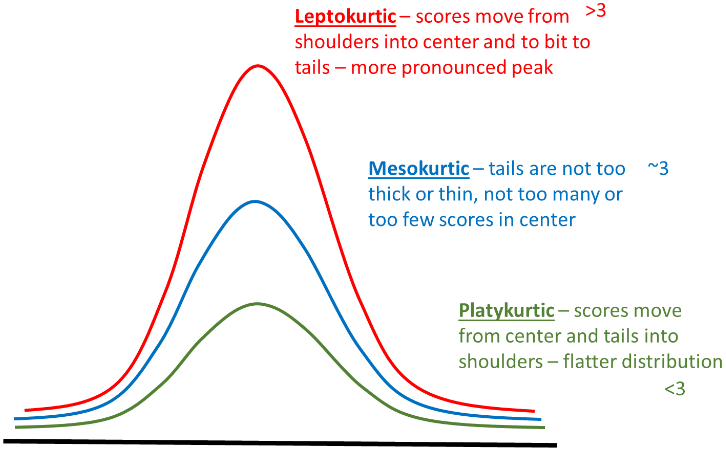
\includegraphics[width=0.8\paperwidth]{../static/course_1_img/forms of kurtosis.PNG}}  
\end{frame}


\begin{frame}
  \frametitle{Volatility Clustering}
  \begin{block}{Definition: Volatility Clustering}
    \begin{itemize}
    \item \textbf{Volatility clustering} means that large price changes (i.e. returns with large absolute values or large squares) occur in clusters
    \item Large price changes tend to be followed by large price changes (up and down)
    \item Periods of tranquility alternate with periods of high volatility (volatility regimes)
    \end{itemize}
    
    \emph{Note: volatility clustering is the consequence of the autocorrelation of the squared returns}\\
    
  \end{block}
\end{frame}


\begin{frame}
  \frametitle{Volatility Regimes: US VIX}
  The VIX is the implied volatility fo the US SP 500:\\ 
  \makebox[\linewidth]{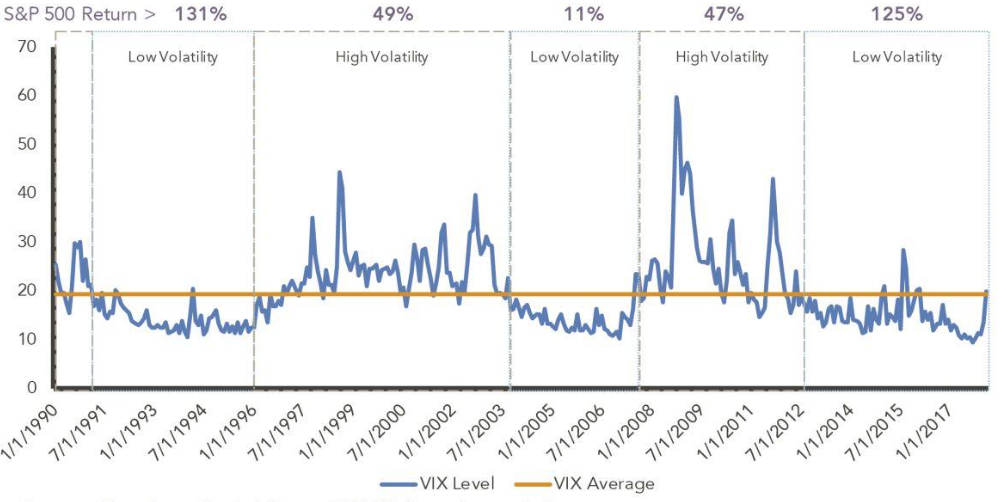
\includegraphics[width=0.8\paperwidth]{../static/course_1_img/vix volatility.PNG}}
  \hspace*{15pt}\hbox{\scriptsize Credit:\thinspace{\scriptsize\itshape Christophe Hurlin}} 
\end{frame}


\begin{frame}
  \frametitle{Aggregational Gaussianity}

  \begin{block}{Definition: Aggregational Gaussianity}
    \begin{itemize}
    \item Asset returns over $k$ days is simply the aggregation of $k$ daily returns
    \item When the time horizon $k$ increases, the central limit theory says that the distribution of returns over a long-time horizon (a few months) tends toward a \textbf{normal distribution}
    \end{itemize}
  \end{block}


  \begin{itemize}
  \item Aggregational gaussianity implies that over long horizons, the pecularities of financial time series over short-term horizon (skewness, kurtosis, etc.) tend to vanish
  \item However, in finance, people are mostly interested in relatively short-term movements, suggesting that working under the gaussianity assumption is often not appropriate
  \end{itemize}
  
\end{frame}


\begin{frame}
  \frametitle{Aggregational Gaussanity In Practice}
  The VIX is the implied volatility fo the US SP 500:\\ 
  \makebox[\linewidth]{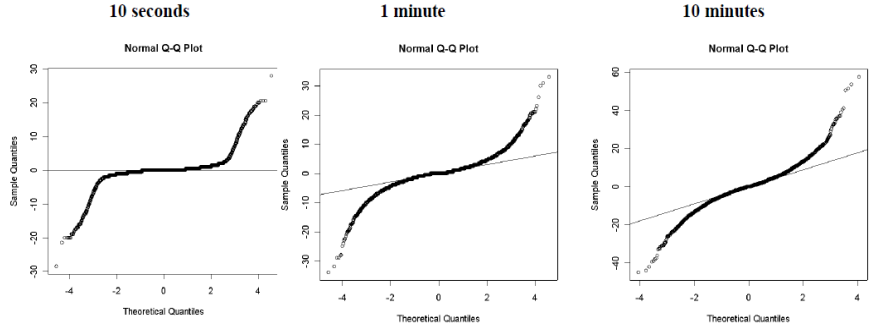
\includegraphics[width=0.8\paperwidth]{../static/course_1_img/aggregational gaussianity.PNG}}
  \hspace*{15pt}\hbox{\scriptsize Credit:\thinspace{\scriptsize\itshape Christophe Hurlin}} 
\end{frame}


\begin{frame}
  \frametitle{Long Range Dependence}
  \begin{block}{Definition}
    \begin{itemize}
    \item At the difference of log returns or standard returns, daily squared returns and absolute returns often exhibit significant autocorrelations
    \item Those autocorrelations are persistent, indicating possible \textbf{long-memory} properties
    \end{itemize}
  \end{block}

\emph{Those autocorrelations become weaker and less persistent when the sampling interval is increased to a week or a month}\\
  
\end{frame}


\begin{frame}
  \frametitle{Long Range Dependence}
  SP 500 Returns (left) and squared returns (right) \\

\medskip
  
 \makebox[\linewidth]{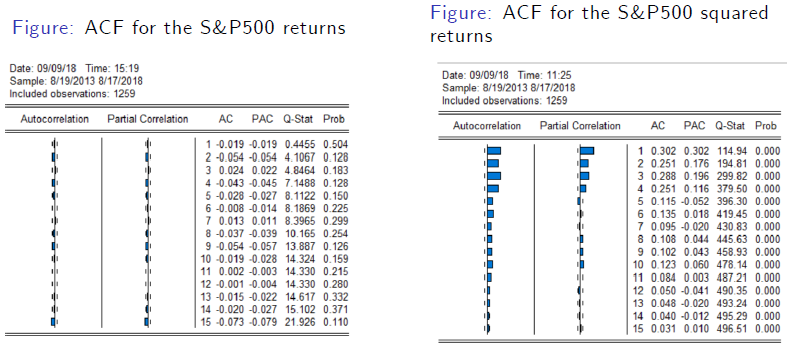
\includegraphics[width=0.8\paperwidth]{../static/course_1_img/long range dependence.PNG}}  
\end{frame}



\begin{frame}
  \frametitle{The ARCH effect}
  \begin{itemize}
  \item The autocorrelation of the squared returns is called the \textbf{ARCH effect} (auto-regressive conditional heteroskedasticity)
  \item It is most important with daily returns, and less important with low frequency returns (monthly, quarterly, etc.)
  \end{itemize}

\medskip
  
ARCH effect is important in finance, because it describes patterns on the dynamic of financial volatility 
  
\end{frame}



\begin{frame}
  \frametitle{Leverage Effect}

  \begin{block}{Definition: the Leverage Effect}
    \begin{itemize}
    \item Assets returns are negatively correlated with the changes in their volatilities
    \item This negative correlation $\text{Corr (returns, vol)}$ is called the \textbf{leverage effect}
    \end{itemize}

Financial explanations
    \begin{itemize}
    \item An asset price declines, companies mechanically become more leveraged (debt-to-equity ratio up) and riskier: therefore, their stock prices become more volatile
    \item On the other hand, when stock prices become more volatile, investors demand high returns and hence stock prices go down
    \item Volatilities caused by price decline are typically larger than prices appreciation due to declined volatilities
    \end{itemize}
    
  \end{block}
  
\end{frame}

\section{Empirical Strategy}

\begin{frame}
  \frametitle{Econometric Model}

  \begin{block}{Definition: Econometric Model}
    An econometric model specificies the statistical relationship between different economic variables, that are expected to be stable over time
  \end{block}

  \begin{enumerate}
  \item \textbf{Parametric model:} fully characterization of the relationship by a \textbf{set of parameters} $\theta$ and a \textbf{link function} $f$ supposed to be known; the specification can be linear or non linear, and includes some randomness $\epsilon$
    \begin{equation*}
      Y = f(X; \theta) + \epsilon
    \end{equation*}

  \item \textbf{Non-parametric and semi-parametric models}: the link function can not be described using a finite number of parameters. The link function is assumed to be unknown and has to be estimated
    
  \item The model is likely to be different from the DGP: there is a \textbf{model risk}
    
  \end{enumerate}
\end{frame}




\begin{frame}
  \frametitle{Example: A Linear Model}

  \begin{exampleblock}{Autoregressive Model: Look at the Past to Forecast the Future}
    A canonical basic time series model is the Autoregressive model of order $p$, called an AR model:

    \begin{equation*}
      X_t = \alpha_0 + \alpha_1 X_{t-1} + \alpha_2 X_{t-2} + \dots + \alpha_p X_{t-p} + \epsilon_t
    \end{equation*}       
  \end{exampleblock}

  \medskip

  \begin{itemize}
  \item $\epsilon_t$ is the randomness in the model: it represents a stochastic element that creates a discrepancy between the model and the reality. The role of a modeler is to reduce this discrepancy as much as possible
  \item The linear model is informative about the \textbf{conditional mean} of $X_t$, i.e. the average value of $X_t$ we can expect given certain past values $\tilde{X}_{t-1}$ of $X_t$
    \begin{equation*}
      \mathbb{E}[X_t|\tilde{X}_{t-1}, \tilde{X}_{t-2}, \dots, \tilde{X}_{t-p}] = \hat{\alpha}_0 + \hat{\alpha}_1 \tilde{X}_{t-1} + \hat{\alpha}_2 \tilde{X}_{t-2} + \dots + \hat{\alpha}_p \tilde{X}_{t-p}  
    \end{equation*}    
  \end{itemize}
  
\end{frame}


\begin{frame}
  \frametitle{How to Specify an Appropriate Time Series Model}
  \begin{wideenumerate}
    \item Study some \textbf{statistical properties} of the observed dat $\{x_t\}$, for instance, the \textbf{stationarity}, the patterns of the autocorrelation function \textbf{ACF}, or the \textbf{partial autocorrelation function}, etc.
    \item Compare these properties to the theoretical properties of some \textbf{typical time series models}, such as AR, MA, ARIMA, SARIMA, etc.
    \item Choose the most appropriate model and \textbf{estimate its parameters}
    \item Use this model for forecasting
  \end{wideenumerate}
\end{frame}


\begin{frame}
  \frametitle{Empirical Strategy}
  The general approach of (financial) econometrics is as follows:\\
  \smallskip

  \begin{wideenumerate}
  \item Specification of the model
  \item Estimation of the parameters
  \item Diagnostic tests
    \begin{itemize}
    \item Significance tests
    \item Specification tests
    \item Backtesting tests
    \item etc.
    \end{itemize}
  \item Interpretation and use of the model (forecasting, historical studies, etc.)
  \end{wideenumerate}
\end{frame}

  \begin{frame}
  \frametitle{Models Family}
  \makebox[\linewidth]{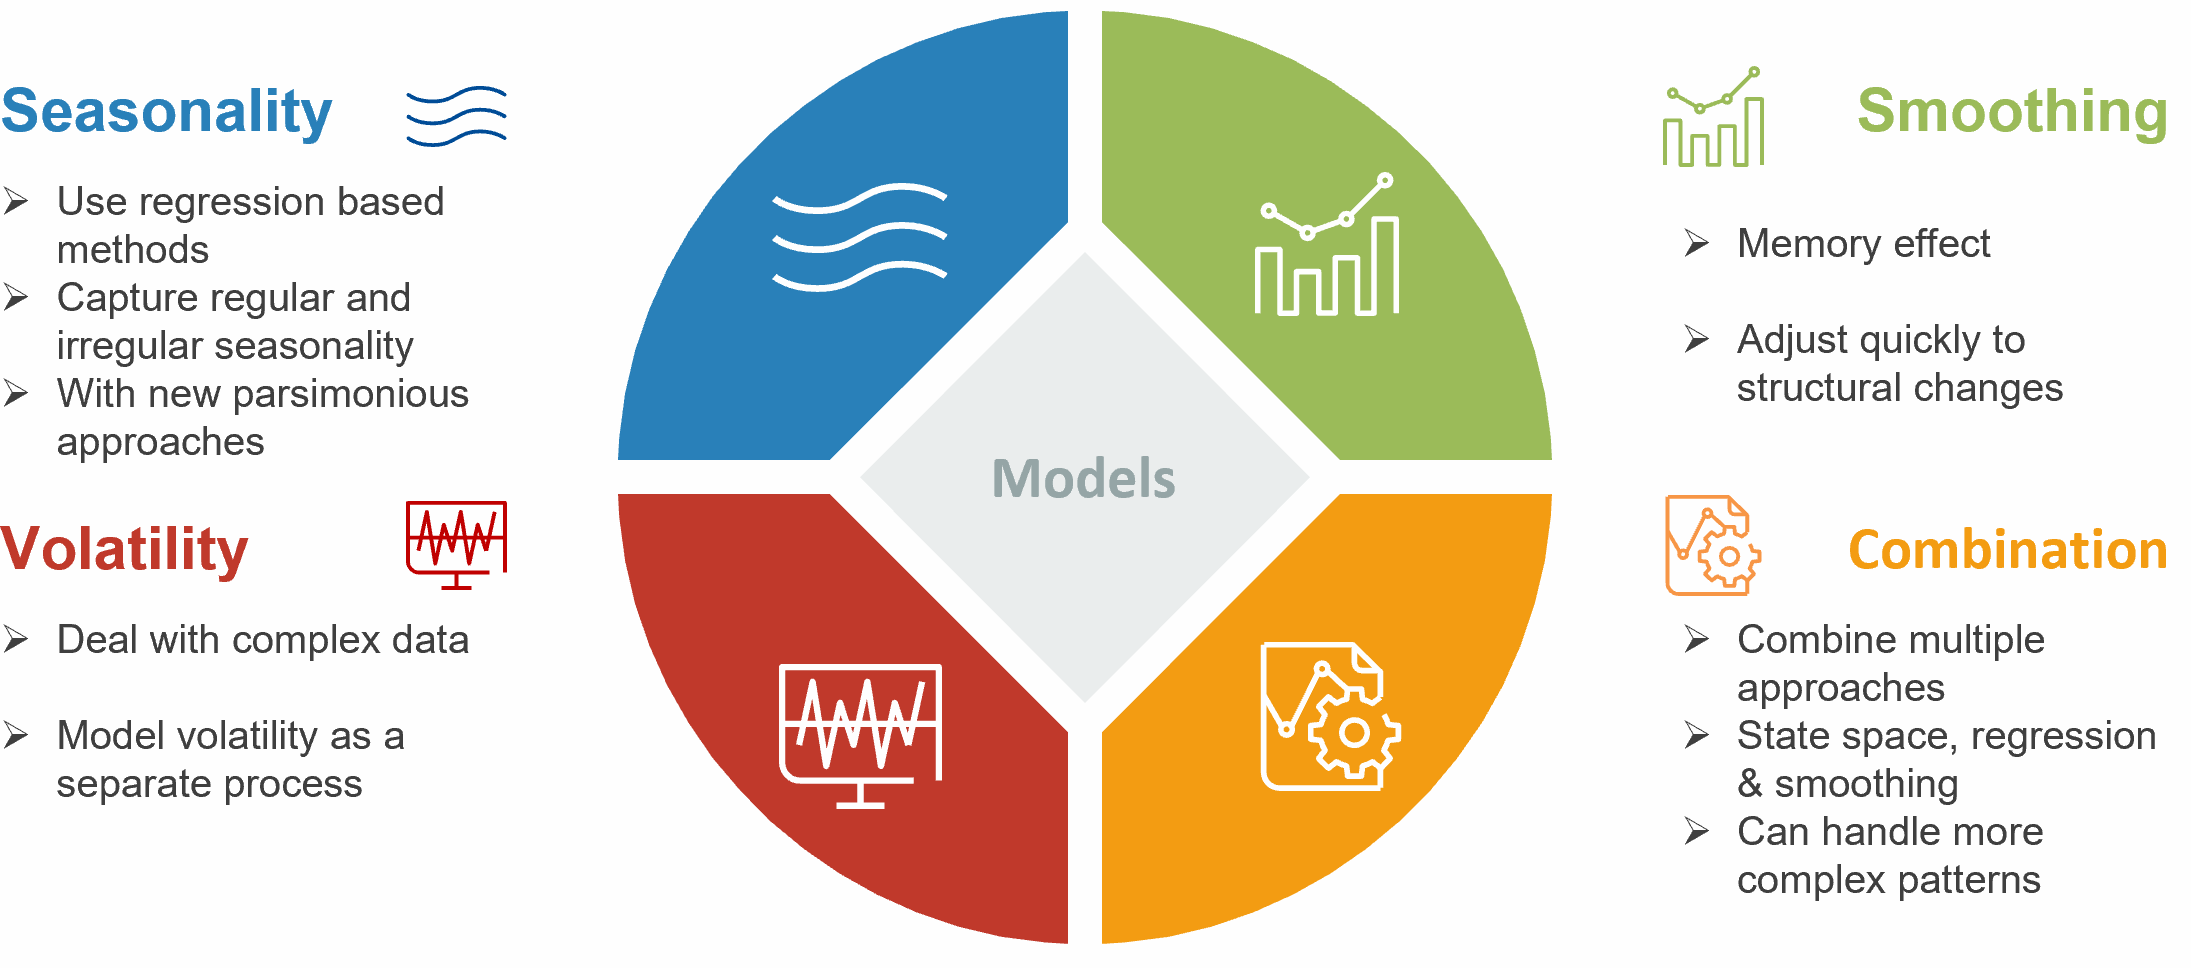
\includegraphics[width=0.85\paperwidth]{../static/course_2_img/models_family.PNG}}
  \hspace*{15pt}\hbox{\scriptsize Credit:\thinspace{\scriptsize\itshape Author}}
\end{frame}


\begin{frame}
  \frametitle{Seasonality in Practice: Currency in Circulation}
  \makebox[\linewidth]{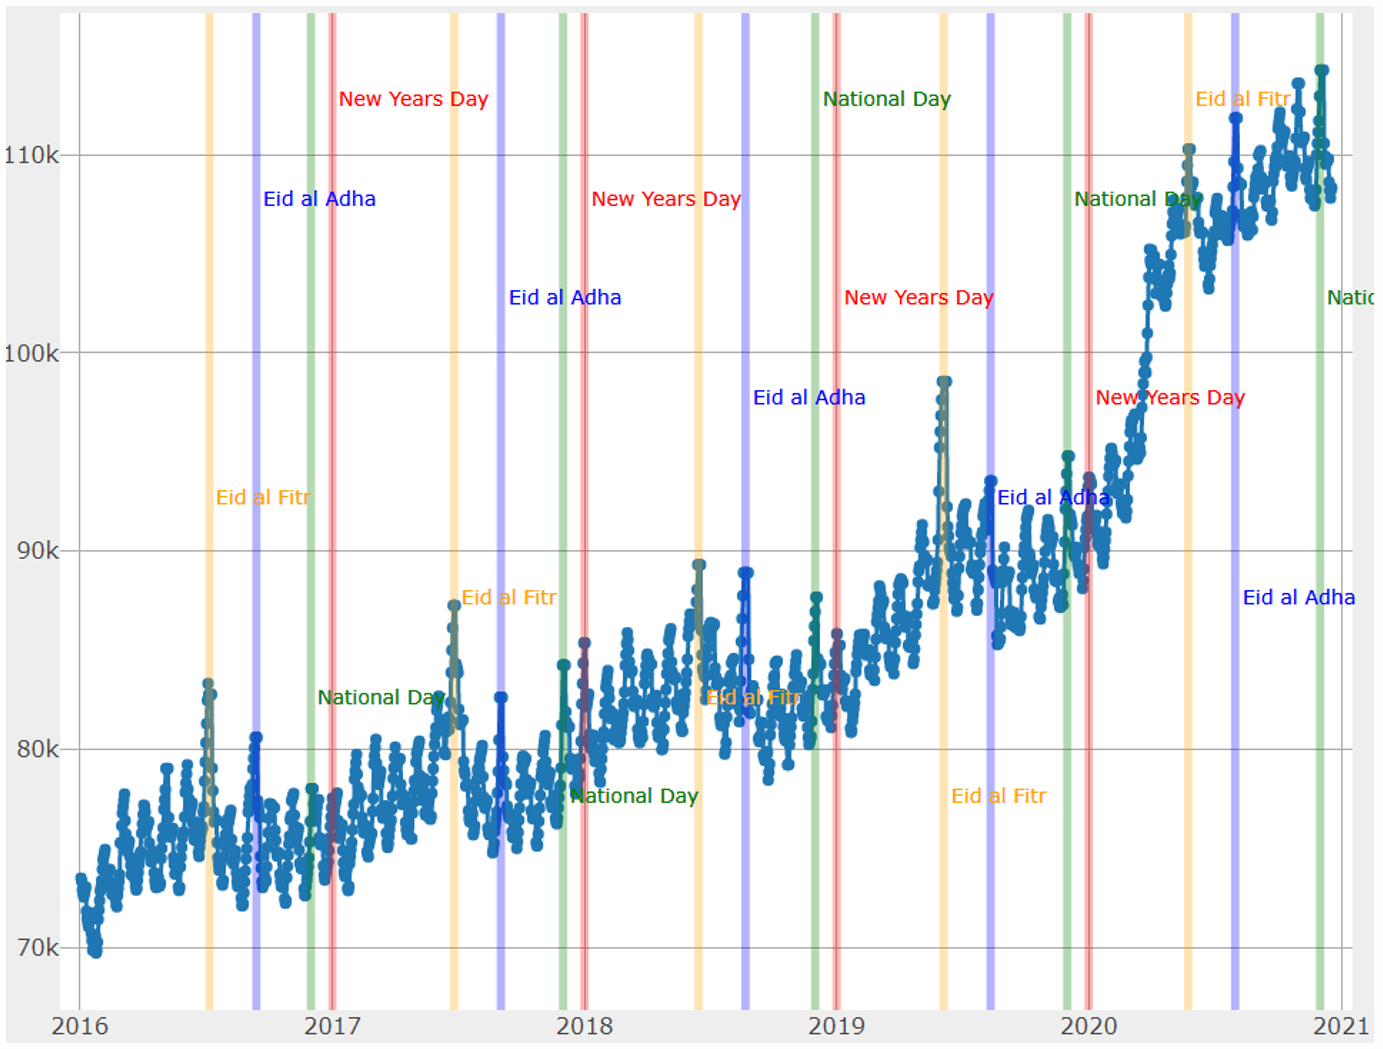
\includegraphics[width=0.75\paperwidth]{../static/course_2_img/seasonal_patterns_practice.PNG}}
  \hspace*{15pt}\hbox{\scriptsize Credit:\thinspace{\scriptsize\itshape IMF TA mission}}
\end{frame}


%% ---------------------------------------------------------------------------
%% Going Deep Into the Models
%% ---------------------------------------------------------------------------
\section{ETS Model}

\begin{frame}
  \frametitle{Exponential Smoothing Patterns}
  \makebox[\linewidth]{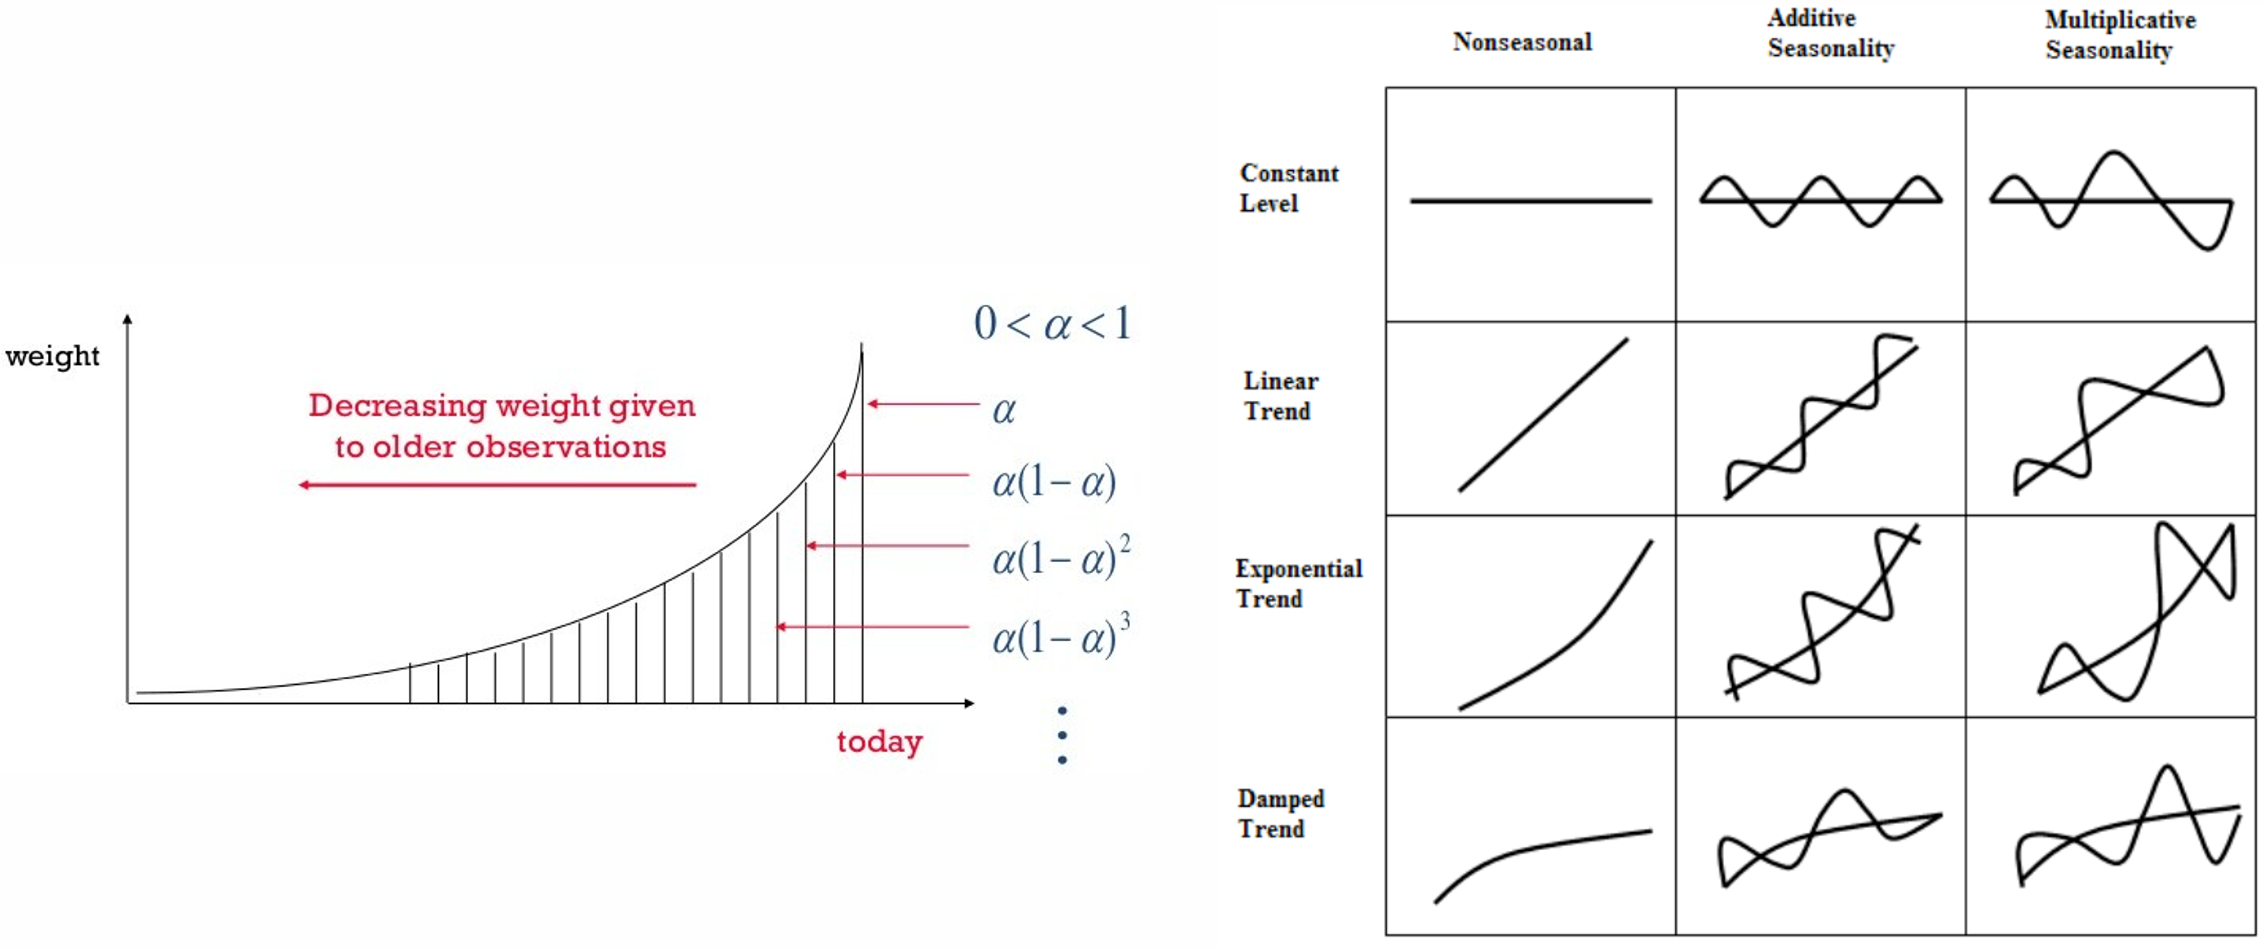
\includegraphics[width=0.85\paperwidth]{../static/course_2_img/exponential_smoothing_patterns.PNG}}
  \hspace*{15pt}\hbox{\scriptsize Credit:\thinspace{\scriptsize\itshape Medium}}
\end{frame}


\begin{frame}
  \frametitle{Perspective}
  
  \begin{itemize}
  \item ETS (Error, Trend, Season) model was developed in the 1950s as algorithms to produce point forecasts
  \item ETS combines a "level" ($l_{t-1}$), a "trend" (($b_{t-1}$)) and a "seasonal" ($s_{t-m}$) components to describe a time series
  \item The combination $f(l_{t-1}, b_{t-1}, s_{t-m})$ can be additive, multiplicative, etc.
  \item The rate of change of the components are controlled by "smoothing" parameters: $\alpha$ for the level, $\beta$ for the trend, $\gamma$ for the seasonal
  \item The researcher has to:
    \begin{enumerate}
    \item To choose the best values for the smoothing parameters 
    \item The initial state of the parameters
    \end{enumerate}
  \item Equivalent ETS state-space models have been developped in the 1990s and the 2000s
  \end{itemize}
  
\end{frame}


\begin{frame}
  \frametitle{Decomposing A Time-Series}
  \makebox[\linewidth]{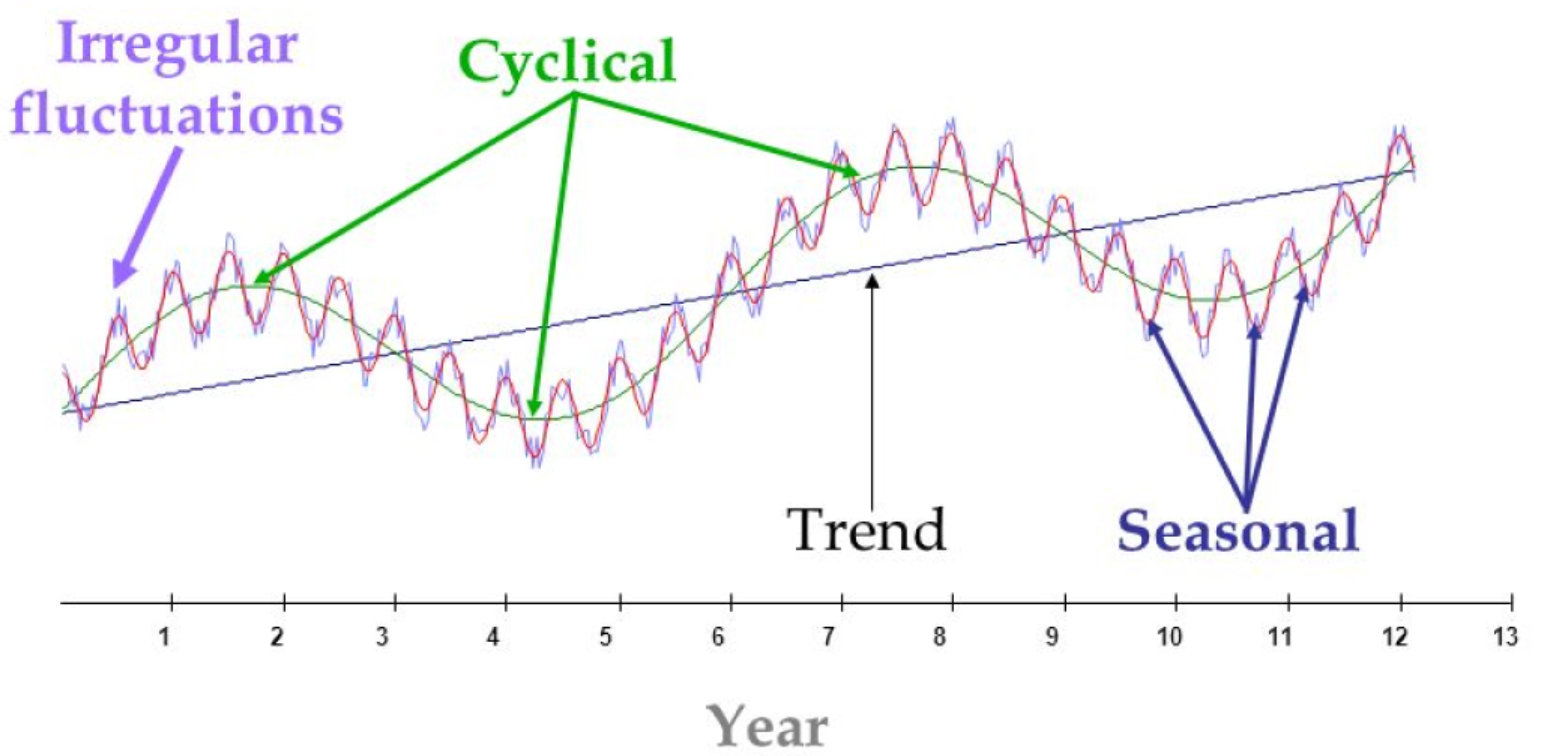
\includegraphics[width=0.75\paperwidth]{../static/course_2_img/time_series_decomposition.PNG}}
  \hspace*{15pt}\hbox{\scriptsize Credit:\thinspace{\scriptsize\itshape medium.com}}
\end{frame}


\begin{frame}
  \frametitle{Combining Level, Trend and Seasonal Components}

  \begin{itemize}
  \item \textbf{Additively:} $y_t = l_{t-1} + b_{t-1} + s_{t-m} + \epsilon_t$
  \item \textbf{Multiplicatively:} $y_t = l_{t-1} \times b_{t-1} \times s_{t-m} \times (1 + \epsilon_t)$
  \item \textbf{Mixed:} $y_t = (l_{t-1} + b_{t-1}) \times s_{t-m} + \epsilon_t $  
  \end{itemize}

  Notations:
  \begin{itemize}
  \item \textbf{Error} can be additive ("A") or multiplicative ("M")
  \item \textbf{Trend} can be None ("N"), additive ("A"), multiplicative ("M") or damped ("Ad" or "Md")
  \item Seasonality can be None ("N"), additive ("A") or multiplicative ("M")
  \end{itemize}
    
\end{frame}


\begin{frame}{Point forecasts and forecast distribution}

  \begin{wideitemize}
  \item Models generates point forecasts estimates, based on a given conditional value $y_{t+1|y0} = f_y(y0)$ 
  \item However, need to generate the forecast distribution to assess the quality of models and select the best. \textbf{Model selection}
  \item A stochastic data generating process (DGP) can generate an entire forecast distribution
  \item Core idea: the residual ($\epsilon$) is the only stochastic (=random) element in $y_t = l_{t-1} + b_{t-1} + s_{t-m} + \epsilon_t$
    \begin{itemize}
    \item Therefore, the distribution of the residuals will determine the distribution of the estimator
    \end{itemize}
  \end{wideitemize}  
\end{frame}


\begin{frame}{Level-Only Model ETS(A, N, N) (Simple Smoothing)}
  \begin{block}{Component Form}
    \begin{itemize}
    \item Forecast equation: $\hat{y}_{t+h |t} = l_t$
    \item Smoothing equation: $l_t = \alpha y_t + (1-\alpha)l_{t-1}$
    \end{itemize}
  \end{block}

  \begin{itemize}
  \item $l_t$ is the level (="smoothed value") of the series at time $t$
  \item $\hat{y}_{t+1|t} = \alpha y_t + (1 - \alpha)\hat{y}_{t|t-1}$
  \end{itemize}
  Iterate to get exponentially weighted moving average form: $\hat{y}_{T+1|T} = \sum_{j=0}^{T-1}\alpha(1-\alpha)^j y_{T-j} + (1-\alpha)^Tl_0$  
\end{frame}

\begin{frame}{Error Correction Form}
  \begin{exampleblock}{Component Form}
    \begin{itemize}
    \item Forecast equation: $\hat{y}_{t+h |t} = l_t$
    \item Smoothing equation: $l_t = \alpha y_t + (1-\alpha)l_{t-1}$
    \end{itemize}
  \end{exampleblock}

  Forecast error: $e_t = y_t - \hat{y}_{t|t-1} = y_t - l_{t-1}$
  
  \begin{block}{Error Correction Form}
    \begin{itemize}
    \item $y_t = l_{t-1} + e_t$
    \item $l_t = l_{t-1} + \alpha*\underbrace{(y_t - l_{t-1})}_{e_t}$
    \end{itemize}

    \begin{itemize}
    \item Intuition: $\alpha$ updates the next-period estimate based on the forecasting error
    \item Specify probability distribution for $e_t$, often assumed that $e_t = \epsilon_t \sim \mathcal{N}(0, \sigma^2)$
    \end{itemize}
           
  \end{block}
  
\end{frame}


\begin{frame}
  \begin{itemize}
  \item Need to choose the best values for $\alpha$ and $l_0$
  \item Similarly to regression, choose optimal parameters by minimizing SSE:
    \begin{equation*}
      \text{SSE} = \sum_{t=1}^T (y_t - \hat{y}_{t|t-1})^2
    \end{equation*}
  \item Unlike regression, there is no closed form solution: need to use numerical optimization
  \end{itemize}
\end{frame}


\begin{frame}{State-Space Representation for Additive Models}
  \begin{alertblock}{State-Space Representation}
    \begin{itemize}
    \item \textbf{Measurement equation}: $y_t = l_{t-1} + \epsilon_t$, where $\epsilon_t \sim \mathcal{N}(0, \sigma^2)$
      \begin{itemize}
      \item The measurement equation is the relationship between observations ($y_t$) and state (=structure) $l_t$
      \end{itemize}
    \item \textbf{State equation} $l_t = l_{t-1} + \alpha*\epsilon_t$, where $\epsilon_t \sim \mathcal{N}(0, \sigma^2)$
      \begin{itemize}
      \item The state equation is evolution of the state variable ($l_t$) through time
      \end{itemize}
     \end{itemize}
  \end{alertblock}


  \begin{itemize}
  \item Both equations have the same error process $\epsilon_t$
  \end{itemize}
  
\end{frame}


\begin{frame}{State-Space Representation for Multiplicative Models}
  \begin{itemize}
  \item Instead of differential errors, specify relative errors: $\eta_t = \frac{y_t - \hat{y}_{t|t-1}}{ \hat{y}_{t|t-1}}$
  \item Some easy algebra, substituting $\hat{y}_{t|t-1} = l_{t-1}$ gives   
  \end{itemize}

  \begin{alertblock}{State-Space Representation}
    \begin{itemize}
    \item \textbf{Measurement equation}: $y_t = l_{t-1}(1+\epsilon_t)$
    \item \textbf{State equation}: $l_t = l_{t-1}(1+\alpha*\epsilon_t)$
    \end{itemize}
  \end{alertblock}

Implication: Models with additivative and multiplicative errors with the same parameters generate \textbf{the same point forecasts but with different prediction intervals}
  
\end{frame}

% Add a few charts

\begin{frame}{Holt's Linear Trend}

  \begin{block}{Component Form}
    \begin{itemize}
    \item Level: $l_t = \alpha_t + (1-\alpha)(l_{t-1}+ b_{t-1})$
    \item Trend: $b_t = \beta*(l_t - l_{t-1}) + (1-\beta)b_{t-1}$
    \item Forecast: $\hat{y}_{t+h|t}=  l_t + hb_t$
    \end{itemize}
  \end{block}

  \begin{itemize}
  \item Two smoothing parameters: $\alpha$ and $\beta$ ($0 \leq \alpha, \ \beta \leq 1$)
  \item $l_t$ level: weighted average between $y_t$ and one-step ahead forecast for time $t$: $l_{t-1} + b_{t-1} = \hat{y}_{t|t-1}$
  \item $b_t$ slope: weighted average of $(l_t - l_{t-1})$ and $b_{t-1}$, current and previous estimate of slope
  \item Choose $\alpha, \ \beta, \ l_0, \ b_0$ to mininize the SSE (sum squared errors)
  \end{itemize}
\end{frame}

% Add a few charts



\begin{frame}{Damped Trend Method}

  \begin{block}{Component Form}
    \begin{itemize}
    \item $l_t = \alpha y_t + (1-\alpha)(l_{t-1} + \phi b_{t-1})$
    \item $b_t = \beta*(l_t - l_{t-1}) + (1-\beta)\phi b_{t-1}$
    \item $\hat{y}_{t+h|t} = l_t + (\phi + \phi^2 + \dots + \phi^h)b_t$
    \end{itemize}
  \end{block}

  \begin{itemize}
  \item $\phi$ is the damping parameter, $0 \leq \phi \leq 1$
  \item If $\phi=1$, the method boils down to Holt's linear trend
  \item As $h \to \infty$, then $\hat{y}_{T+h|T} \ \to \ l_T + \frac{\phi b_T}{1-\phi}$
  \item Application: short-run forecasts are trended, long-run forecasts constant
  \end{itemize}
  
  
\end{frame}


\begin{frame}{Holt-Winters Seasonal Model}

  Holt and Winters extended Holt's method to capture seasonality
  
  \begin{block}{Component Form}
    \begin{itemize}
    \item Level: $l_t = \alpha (y_t - s_{t-m}) + (1- \alpha )(l_{t-1} + b_{t-1})$
    \item Trend: $b_t = \beta(l_t - l_{t-1}) + (1-\beta)b_{t-1}$
    \item Season: $\gamma(y_t - l_{t-1} - b_{t-1}) + (1-\gamma)s_{t-m}$
    \item Forecast: $\hat{y}_{t+h|t} = l_t + hb_t + s_{t+h - m(k+1)}$
    \end{itemize}
  \end{block}

  \begin{itemize}
  \item $m$ is the period of seasonality (e.g. $m = 4$ for quarterly data)
  \end{itemize}
  
\end{frame}


\begin{frame}{Seasonal Component}
  \begin{itemize}
  \item The seasonal component is usually expressed as:
    \begin{equation*}
      s_t = \gamma*(y_t - l_t) + (1-\gamma)*s_{t-m} \qquad 0 \ \leq \ \gamma \ \leq 1
    \end{equation*}
  \item By subtitution, we can derive the dynamic of the seasonal term as:
    \begin{equation*}
      s_t = \gamma*(1-\alpha)(y_t - l_{t-1} - b_{t-1}) + [1 - \gamma(1-\alpha)] s_{t-m}
    \end{equation*}
  \end{itemize}  
\end{frame}




\begin{frame}{Forecasting with ETS models}
\textbf{Traditional point forecasts}: iterate the equations for $t = T+1, T+2, \dots, T+h$. By construction, $\epsilon_t = 0 \ \forall \ t>T$

\begin{wideitemize}
\item Equals to $E[y_{t+h}|x_t]$ in the case of additive seasonality only
\item Point forecasts for additive ETS are the same as for multiplicative ETS if the parameters are the same
\end{wideitemize}
  
\end{frame}



\begin{frame}{Prediction Intervals}

  \begin{wideitemize}
  \item They can only be generated using the models
  \item The prediction intervals will differ between models with additive and multiplicative errors
  \item Some simple ETS models offer exact formula
  \item For more complex ETS models, the only solution for generating the confidence intervals is by bootstrapping
    \begin{itemize}
    \item Simulate future sample paths, conditional on the last estimates of the states
    \item Obtain the prediction intervals from the percentiles of these simulated future paths
    \end{itemize}
  \end{wideitemize}
  
\end{frame}


\begin{frame}
  \frametitle{Main Idea: Control the Rate of Change}

  \begin{wideitemize}
  \item $\alpha$ controls the flexibility of the \textbf{level}
    \begin{itemize}
    \item If $\alpha = 0$, the level never updates (stays at the mean)
    \item If $\alpha = 1$, the level updates completely (naive, start from yesterday)
    \end{itemize}
  \item $\beta$ controls the flexibility of the \textbf{trend}
    \item If $\beta = 0$, the trend is linear
    \item If $\beta = 1$, the trend changes suddenly at each observation
    
    \item $\gamma$ controls the flexibility of the \textbf{seasonality}
      \begin{itemize}
      \item If $\gamma = 0$ the seasonality is fixed (seasonal mean)
      \item If $\gamma = 1$ the seasonality updates completely (seasonal naive)        
      \end{itemize}
  \end{wideitemize}
  
\end{frame}

\begin{frame}
  \frametitle{Stability and Forecastability}
  \begin{wideitemize}
  \item Stability and forecastability have deep mathematical implications that I will only explain intuitively\\

    \smallskip
    
    \begin{itemize}
    \item \textbf{Stability:} the weights of the observations decay over time, guaranteeing that the newer ones will have higher weights than old one.
      \begin{itemize}
      \item \emph{This is the core principle behind exponential weights: the model captures information update as time goes through}. 
      \end{itemize}

      \smallskip
      
    \item \textbf{Forecastability:} The forecastability does not guarantee that the weights decay, but it guarantees that the initial value of the state vector will have a constant impact on forecasts, i.e. will not increase in weight with the increase of the forecast horizon.
      \begin{itemize}
      \item \emph{Forecastability is a variation around the concept of ergodicity: it implies that, as the model embedds new observations, the impact of "old information" from the old observations does not "pollute" the new information brought by the new observations. In other words, the model is "learning" relevant information }
      \end{itemize}
    \end{itemize}
    \item More information: \url{https://otexts.com/fpp3/}
  \end{wideitemize}
\end{frame}


\section{ARIMA Models}


\begin{frame}{ARIMA Model}

  \begin{itemize}
  \item AR: autoregressive (lagged observations as inputs)
  \item I: integrated (differencing to make series stationary)
  \item MA: moving average (lagged errors as inputs)
  \end{itemize}

  \begin{block}{Intuition}
    Contrary to an ETS, an ARIMA model is rarely interpretable in terms of visible data structures like trend and seasonality. But it can capture a huge range of time series patterns
  \end{block}  
\end{frame}


\begin{frame}{Refresher: Intuitive Definition of Stationarity}

  \begin{block}{Intuitive Characterization}
    If ${y_t}$ is a stationary time series, then for any period $s$ in the future, the distribution $\{y_t, \dots, y_{t+s}\}$ doesn't depend on $t$
  \end{block}

  A \textbf{stationary series} is:
  \begin{itemize}
  \item Roughly horizontal
  \item Constant variance
  \item No predictable patterns in the long term
  \end{itemize}

  Stabilization: 
  \begin{itemize}
  \item Transformations help to \textbf{stabilize the variance}
  \item For ARIMA modelling, we also need to \textbf{stabilize the mean}
  \end{itemize}
  
\end{frame}


\begin{frame}{Identifying Non-Stationary Series}

  Tips:\\
  
  \begin{wideitemize}
  \item Time plot
  \item The ACF of stationary data drops to zero relatively quickly
  \item The ACF of non-stationary data decreases slowly
  \item For non-stationary data, the value of the first coefficient is often large and positive
  \end{wideitemize}

  
\end{frame}


\begin{frame}
  \frametitle{Stationary?}
     \makebox[\linewidth]{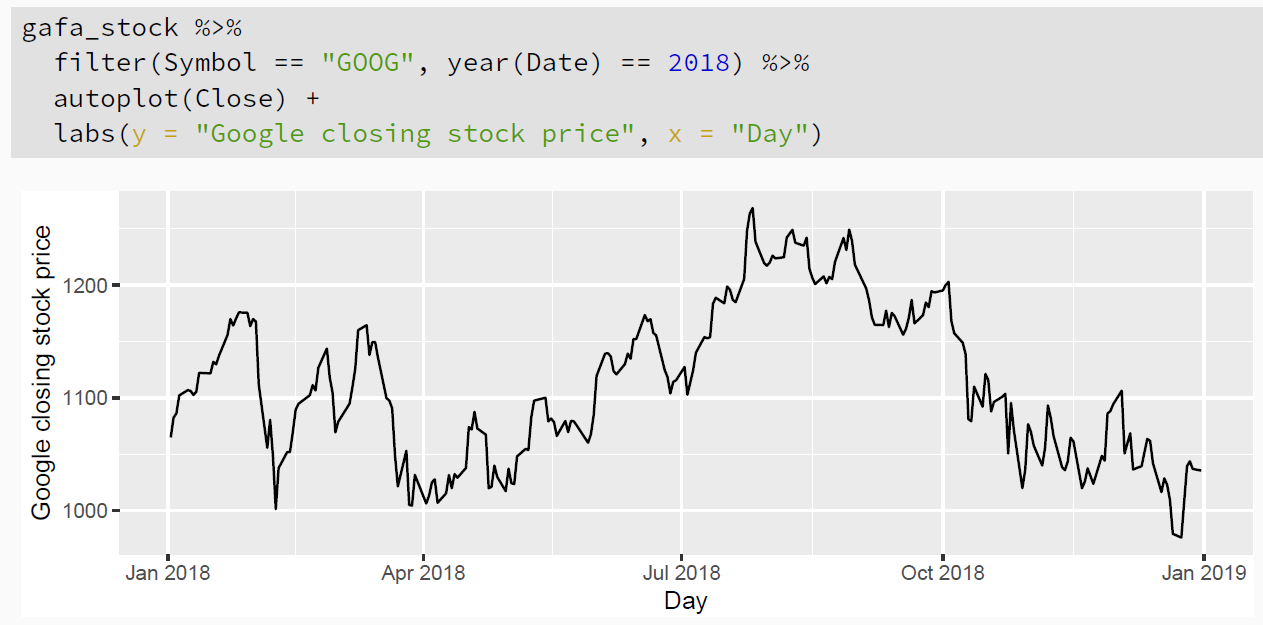
\includegraphics[width=0.95\paperwidth]{../static/course_2_img/google_price.PNG}}  
\end{frame}


\begin{frame}
  \frametitle{Stationary?}
     \makebox[\linewidth]{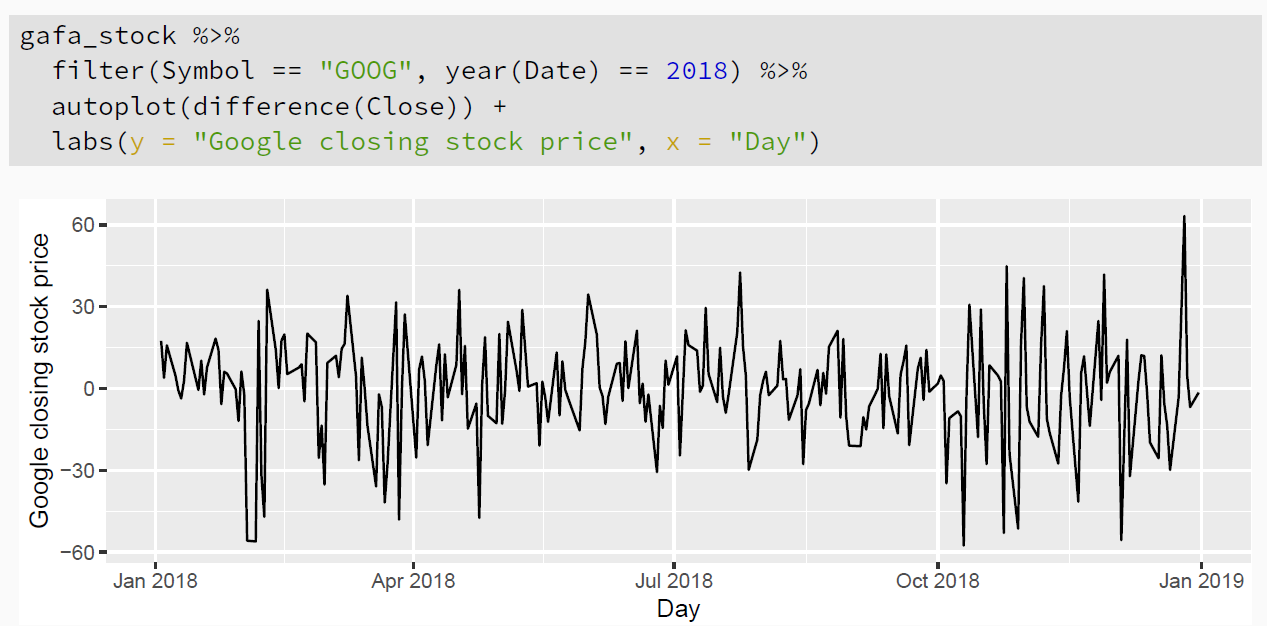
\includegraphics[width=0.95\paperwidth]{../static/course_2_img/google_price_first_diff.PNG}}  
\end{frame}

\begin{frame}
  \frametitle{Stationary?}
     \makebox[\linewidth]{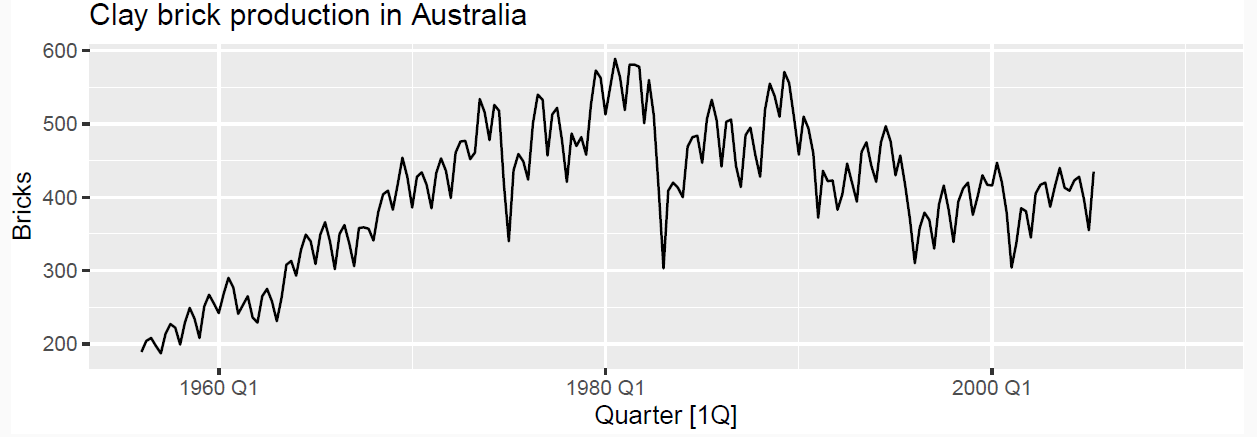
\includegraphics[width=0.95\paperwidth]{../static/course_2_img/clay_brick.PNG}}  
\end{frame}


\begin{frame}{Differencing}
  \begin{wideitemize}
  \item Differencing helps to \textbf{stabilize the mean}
  \item The differenced series is the \emph{change} (or first difference) between each observation in the original series: $y'_t = y_t - y_{t-1}$
  \item The differenced series will have only $T-1$ values since it is not possible to calculate a difference $y'_1$ for the first observation
  \end{wideitemize}

\end{frame}


\begin{frame}{Random Walk Model}
  If the differenced series is white noise with zero mean:
  \begin{block}{Specification}
    \begin{equation*}
      y_t - y_{t-1} = \epsilon_t \qquad \text{where} \ \epsilon_t \ \sim \ \mathcal{N}(0, \sigma^2)
    \end{equation*}
  \end{block}

  \begin{itemize}
  \item Very widely used for non-stationary data
  \item This is the model behind the \textbf{naive method}
  \item Random walks typically have:
    \begin{itemize}
    \item Long periods of apparent trends up or down
    \item Sudden/unpredictable chanes in direction
    \end{itemize}
  \item In a random walk, the forecast are equal to the last observation
    \begin{itemize}
    \item Future movements up or down are equally likely
    \end{itemize}
  \end{itemize}   
\end{frame}


\begin{frame}{Random Walk with Drift Model}
  If the differenced series has a drift $c$:

  \begin{equation*}
    y_t - y_{t-1} = c + \epsilon_t \qquad \text{where} \ \epsilon_t \ \sim \ \mathcal{N}(0, \sigma^2)
  \end{equation*}
  
  \begin{wideitemize}
  \item $c$ is the \textbf{average change} between consecutive observations
  \item If $c > 0$, $y_t$ will tend to drift upwards and vice-versa
  \item This is the model behind the \textbf{drift method} 
  \end{wideitemize}  
\end{frame}



\begin{frame}{Second-Order Differencing}

  Occasionally, the differenced data will not appear stationary and it may be necessary to difference the data a second time:\\

  \medskip
  
  \begin{equation*}
    y''_{t} = y'_t - y'_{t-1} = (y_t - y_{t-1}) - (y_{t-1} - y_{t-2})
  \end{equation*}

  \medskip

  \begin{itemize}
  \item $y''_{t}$ will have $T-2$ values
  \item In practice, it is almost never necessary to go beyond second-order differences
  \end{itemize}
  
\end{frame}


\begin{frame}{Seasonal Differencing}

  \begin{block}{Definition: Seasonal Difference}
    A seasonal difference is the difference between an observation and the corresponding observation from the previous year

    \begin{equation*}
      y'_t = y_t - y_{t-m}
    \end{equation*}

    where $m$ = number of seasons


    \begin{itemize}
    \item For monthly data, $m = 12$
    \item For quarterly data, $m = 4$      
    \end{itemize}
    
  \end{block}
\end{frame}


\begin{frame}{Differencing in Practice}

  When both seasonal and first differences are applied:

  \begin{wideitemize}
    \item It makes no difference which one is done first - the result will be the same
    \item If seasonality is strong, we recommend that seasonal differencing be done first because sometimes the resulting series will be stationary and there will be no need for further first difference
    \item It is important that, if differencing is used, the differences are \textbf{interpretable}: for instance, taking lag 3 differences for yearly data is difficult to interpret
  \end{wideitemize}
\end{frame}


\begin{frame}{Unit Root Tests}
  Statistical tests can be used to determine the required order of differencing\\

  \smallskip

  \begin{wideenumerate}
    \item \textbf{Augmented Dickey Fuller test}: null hypothesis is that the data is non-stationary and non-seasonal
    \item KPSS (Kwiatkowski-Phillips-Schmidt Shin) test: the null hypothesis is that the data is stationary is non-seasonal
    \item Other tests are available for seasonal data
  \end{wideenumerate}
  
  
\end{frame}



\begin{frame}{Backshift Notation}

  \begin{block}{Notation}
    The backshift notational device, $B$ is used as follows:\\

    \begin{equation*}
      B y_t = y_{t-1}
    \end{equation*}
  \end{block}

    
    \begin{itemize}
    \item   $B$ operating on $y_t$ has the effect of \textbf{shifting the data back one period}
    \item   Two applications of $B$ to $y_t$ shifts the data back \textbf{two periods}
      \begin{equation*}
        B(By_t) = B^2 y_t = y_{t-2}
      \end{equation*}
    \end{itemize}
    
$B$ depends on the period/frequency considered. Shifting monthly data by a year supposes using $B^{12}$

\end{frame}


\begin{frame}{Relationship with Differencing}
  Importantly, the backshift operator is convenient for describing differencing\\

  \medskip
  
  \begin{exampleblock}{Backshift Operator and Differencing}
    $$y'_t = y_t - y_{t-1} = y_t - By_t = (1-B)y_t$$
  \end{exampleblock}


  \begin{itemize}
    \item Likewise, second-order differences are obtained with: $y''_t = (1-B)^2y_t$  
    \item Pay attention !! Second-order difference is not second difference 
      \begin{itemize}
      \item Second order difference: $(1-B)^2 y_t = y''_t = (y_t - y_{t-1}) - (y_{t-1} - y_{t-2})$
      \item Second difference: $1-B^2 y_t = y_t - y_{t-2}$
      \end{itemize}
  \end{itemize}
  
\end{frame}


\begin{frame}{Combined Effects}

Assume that you want to combine a first difference with a seasonal difference:
  
  \begin{itemize}
  \item First difference: $(1-B)$
  \item Seasonal difference: $(1-B^m)$
  \end{itemize}

  Then, the backshift operator can be directly combined, as a polynomial, to represent the transformed time series:

  \begin{equation*}
    (1-B)(1-B^m)y_t = (1 - B - B^m + B^{m+1})y_t = y_t - y_{t-1} - y_{t-m} + y_{t-m-1}
  \end{equation*}    
\end{frame}


\begin{frame}
  \frametitle{Autoregressive (AR) Models}

  \begin{block}{Definition}
    \begin{equation*}
      y_t = c + \phi_1 y_{t-1} + \phi_2 y_{t-2} + \dots + \phi_P y_{t-p} + \epsilon_t
    \end{equation*}

    \begin{itemize}
    \item where $\epsilon_t$ is a white noise
    \item This is a multiple regression with \textbf{lagged variables}
    \end{itemize}    
  \end{block}

  \makebox[\linewidth]{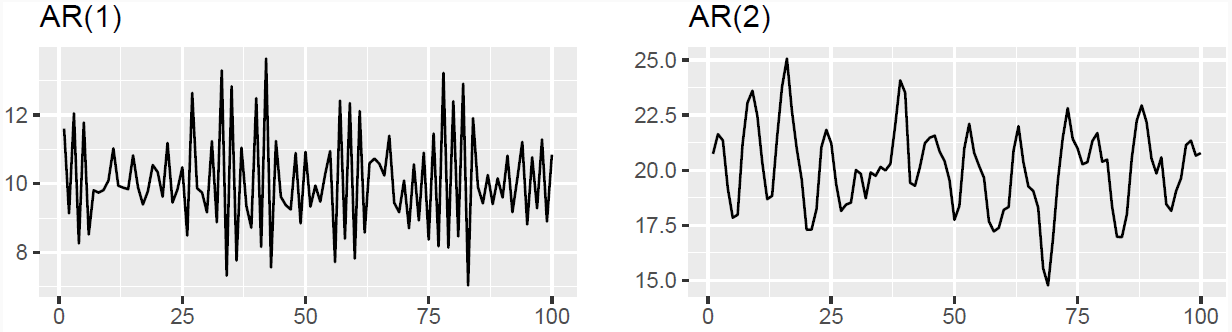
\includegraphics[width=0.7\paperwidth]{../static/course_2_img/ar1_ar2.PNG}}   
\end{frame}


\begin{frame}
  \frametitle{AR(1) Model}
  \begin{block}{Specification}
    \begin{equation*}
      y_t = c + \phi_1 y_{t-1} + \epsilon_t
    \end{equation*}
  \end{block}

  \begin{itemize}
  \item When $\phi_1=0$, $y_t$ is equivalent to a \textbf{white noise}
  \item When $\phi_1=1$ and $c=0$, $y_t$ is equivalent to a \textbf{random walk}
  \item When $\phi_1=1$ and $c \neq 0$, $y_t$ is equivalent to a \textbf{random walk with drift}
  \item When $\phi_1<0$ $y_t$ tends to oscillate between positive and negative values 
  \end{itemize}
  
\end{frame}


% Add charts

\begin{frame}
  \frametitle{Stationarity Conditions}
  To restrict AR models to stationary data, some contraints on the coefficients are needed

  \begin{alertblock}{General Condition for Stationarity}
    Complex roots of the polynomial $\mathcal{P}(z) = 1 - \phi_1z - \phi_2 z^{2} - \dots \phi_p z^{p}$ lie outside the unit circle of the complex plane
  \end{alertblock}

  \begin{wideitemize}
  \item Intuition: For an AR(1) model, the backshift polynomial is $y_t = \phi_1 y_{t-1} + \epsilon_t \ \leftrightarrow \ y_t(1-\phi_1B) = \epsilon_t$
  \item $(1-\phi_1B) = 0 \ \leftrightarrow \ B= \underbrace{\frac{1}{\phi_1}}_{\text{Not explosive}}$
  \item To get the AR expression not explosive, we need $|\frac{1}{\phi_1}| < 1$ and therefore $|\phi_1| > 1$ 
  \end{wideitemize}


  \end{frame}


\begin{frame}
  \frametitle{The Case for Low Lags Orders}

  For low lags orders, the stationarity conditions are simply:\\
  
  \begin{wideitemize}
  \item For $p=1$: $-1 < \phi_1 < 1$
  \item For $p=2$:  $-1 < \phi_2 < 1$, $ \phi_1 + \phi_2 < 1$ and $ \phi_2 - \phi_1 < 1$
  \item More complex conditions hold for $p \geq 3$
  \item Estimation software (R, Python, Eviews, etc.) takes care of this
  \end{wideitemize}
  
\end{frame}



\begin{frame}
  \frametitle{Moving Average Model}
  \begin{block}{Definition: Moving Average Model}
    \begin{equation*}
      y_t = c + \epsilon_t + \theta_1 \epsilon_{t-1} + \theta_2 \epsilon_{t-2} + \dots + \theta_q \epsilon_{t-q}
    \end{equation*}
    \begin{itemize}
    \item $\epsilon_t$ is a white noise
    \item This is a multiple regression with \textbf{past errors} as predictors
    \item Do NOT confuse this with \emph{moving average smoothing}!
    \end{itemize}    
  \end{block}

  \makebox[\linewidth]{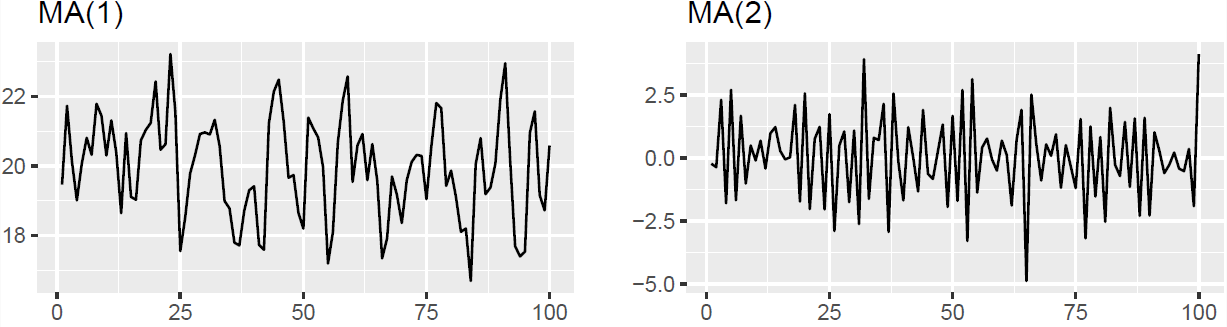
\includegraphics[width=0.7\paperwidth]{../static/course_2_img/ma1_ma2.PNG}}     
\end{frame}



\begin{frame}
  \frametitle{Wold Decomposition: From AR(p) to MA($\infty$) Model}

  \begin{block}{Wold Decomposition}
    It is possible to write any \textbf{stationary} AR(p) model as an MA($\infty$)
  \end{block}

  \begin{itemize}
  \item Intuitive: just go backward!
  \item $y_t = \phi_1 \underbrace{y_{t-1}}_{} + \epsilon_t$
  \item $y_t = \phi_1 (\phi_1 y_{t-1} + \epsilon_{t-1}) + \epsilon_t$ = $\phi_1^2 y_{t-2} + \phi_1\epsilon_{t-1} + \epsilon_t$
  \item $\dots$
  \item Providing that $1 < \ \phi_1 \ < 1$:
    \begin{equation*}
      y_t = \epsilon_t + \phi_1 \epsilon_{t-1} + \phi_1^2 \epsilon_{t-2} + \phi_1^3 \epsilon_{t-3} + \dots
    \end{equation*}
  \end{itemize}  
\end{frame}


\begin{frame}
  \frametitle{Invertibility: From MA(q) to AR($\infty$)}

  \begin{wideitemize}
    \item Under certain conditions, an MA(q) process can be written as an AR($\infty$) process
    \item In this case, the MA model is said to be \textbf{invertible}
    \item Invertible models have some mathematical properties that make them easier to use in practice
    \item Invertability of an MA model is equivalent to the \textbf{forecastability} of an ETS model
      \begin{itemize}
      \item This is intuitive: AR processes are embedding new information on the most recent lags 
      \end{itemize}
  \end{wideitemize}
  
\end{frame}


\begin{frame}
  \frametitle{Invertibility}

  \begin{alertblock}{General Condition for MA(q) Invertibility}
    Complex roots of $1 + \theta_1z + \theta_2 z^2 + \dots + \theta_q z^q$ lie outside the unit circle of the complex plane
  \end{alertblock}

  \smallskip

  \begin{itemize}
  \item For q =1: $-1 \ < \theta_1 \ <1$
  \item For q=2:
    \begin{itemize}
    \item $-1 \ < \theta_2 \ <1$
    \item $\theta_1 + \theta_2 > -1$ and $\theta_1 - \theta_2 \ < 1$
    \end{itemize}
  \item More complicated solutions hold for $q \geq 3$
  \item Estimation software takes care of this
  \end{itemize}
  
\end{frame}


\begin{frame}
  \frametitle{ARMA(p, q) Model}
  \begin{block}{Specification}
    \begin{equation*}
      y_t = c + \underbrace{\phi_1 y_{t-1} + \dots + \phi_p y_{t-p}}_{\text{AR}} + \underbrace{\theta_1 \epsilon_{t-1} + \dots + \theta_q \epsilon_{t-q}}_{\text{MA}} + \epsilon_t
    \end{equation*}
  \end{block}

  \medskip

  \begin{itemize}
  \item The predictors include both \textbf{lagged values of $y_t$} and \textbf{lagged errors}
  \item Important specification: the future value of the series depends both on the past values it took (dynamic), as well as recent random noise / error term 
  \item This simple model is "learning" both from the dynamic of the past values and from its inherent randomness
  \item Conditions on AR coefficients ensure \textbf{stationarity}
  \item Conditions on MA coefficients ensure \textbf{invertibility}
  \end{itemize}
  
\end{frame}

\begin{frame}
  \frametitle{Autoregressive Integrated Moving Average (ARIMA)}

  ARIMA: AR\textbf{I}MA stands for: Autoregressive \textbf{Integrated} Moving Average model

  \begin{itemize}
  \item Basically, it is a non-stationary model that can be made stationary by differencing
  \item $(1-B)^d y_t$ follows an ARMA model: $d$ is the degree of differencing
  \item Once differenced $d$ times, it is stationary and behaves as an ARMA model
  \end{itemize}  
\end{frame}


\begin{frame}
  \frametitle{Generalization}

  \begin{wideitemize}
  \item $ARIMA(p, d, q)$ where $p$ is the autoregressive order, $d$ the degree of differencing and $q$ the order of the moving average part
  \item All linear models we discussed are special cases of the ARIMA model:
    \begin{wideitemize}
    \item White noise model: $ARIMA(0, 0, 0)$
    \item Random walk: $ARIMA(0, 1, 0)$ with no constant
    \item Random walk with drift: $ARIMA(0, 1, 0)$ with constant  
    \item $AR(p) = ARIMA(p, 0, 0)$ , $MA(q) = ARIMA(0, 0, q)$
    \end{wideitemize}
  \end{wideitemize}
    
\end{frame}



\begin{frame}
  \frametitle{Backshift Notation for ARIMA}
  ARIMA(1, 1, 1) model:

  \begin{equation*}
    \underbrace{(1-\phi_1B)}_{AR(1)} \ \underbrace{(1-B)y_t}_{\text{First difference}} \quad = \quad c + \underbrace{(1+\theta_1B)\epsilon_t}_{MA(1)}
  \end{equation*}  
\end{frame}



\begin{frame}
  \frametitle{ARIMA Analysis with Egyptian Exports}
  \makebox[\linewidth]{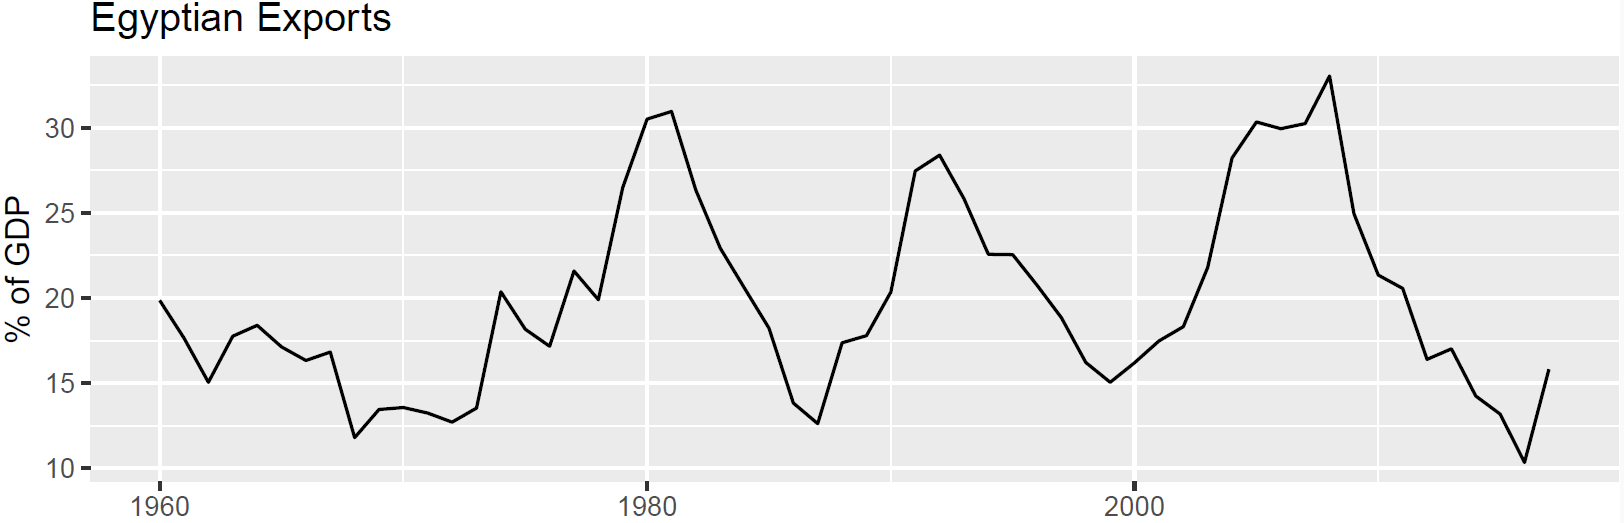
\includegraphics[width=0.95\paperwidth]{../static/course_2_img/egyptian_exports.PNG}}     
\end{frame}


\begin{frame}
  \frametitle{Egyptian Exports Fit}
  \makebox[\linewidth]{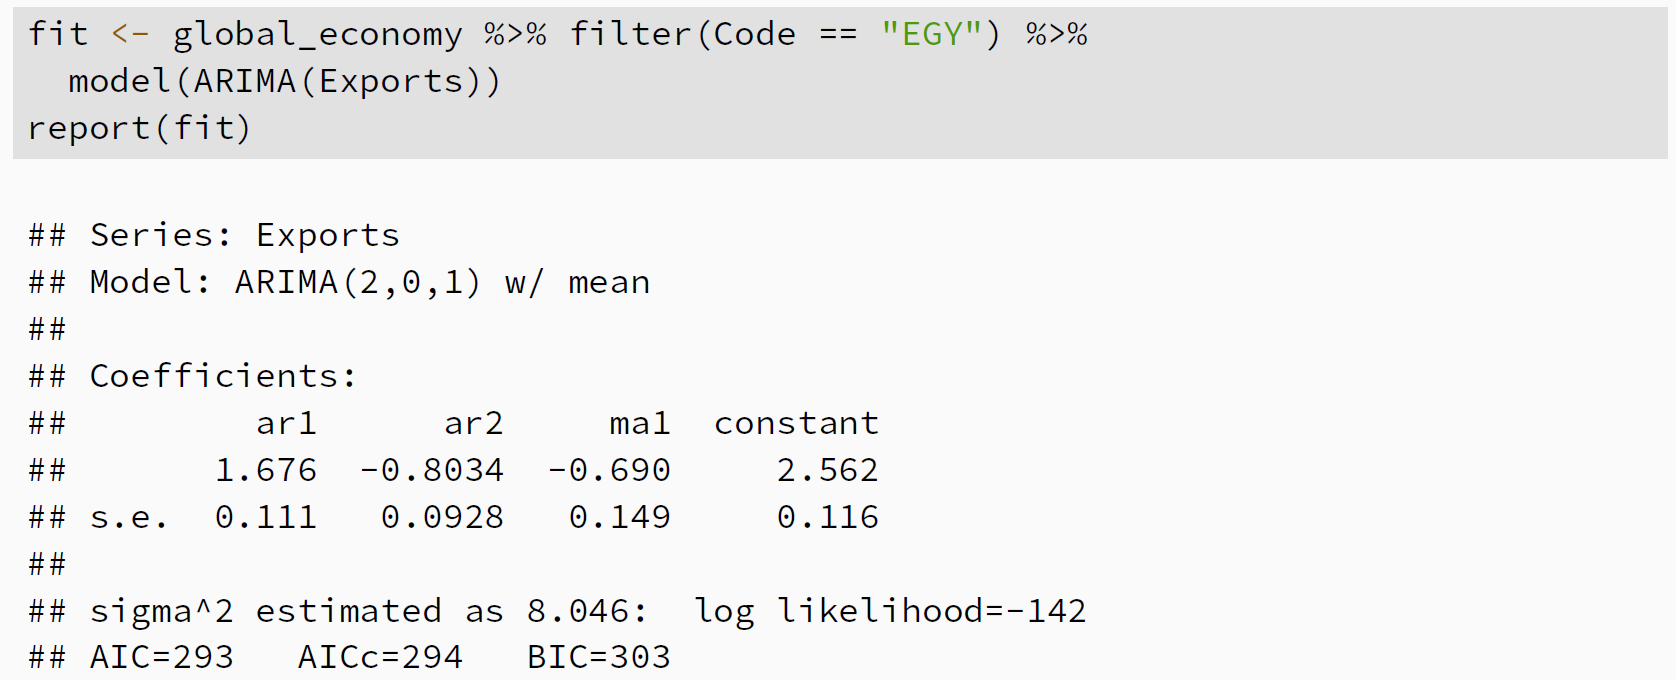
\includegraphics[width=0.95\paperwidth]{../static/course_2_img/egyptian_exports_fit.PNG}}     
\end{frame}

\begin{frame}
  \frametitle{Egyptian Exports Fit Residuals}
  \makebox[\linewidth]{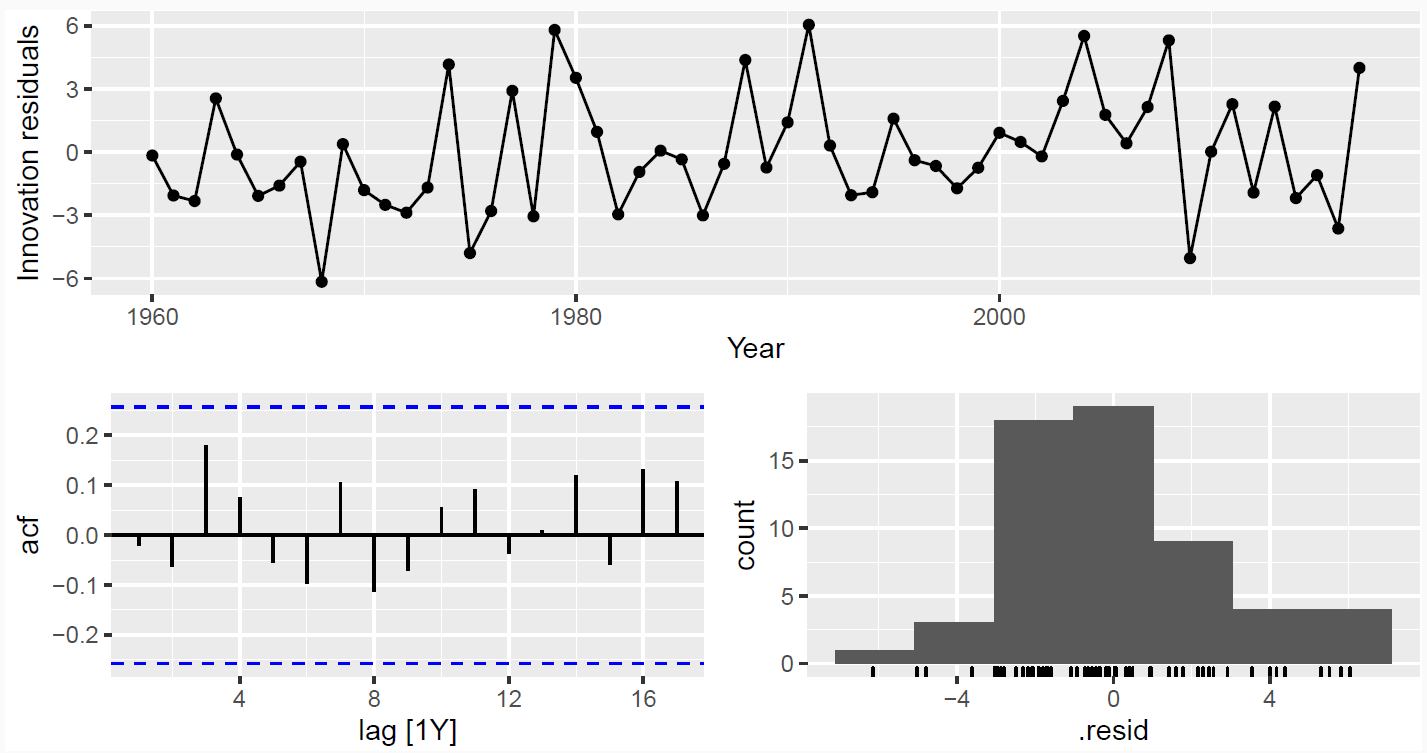
\includegraphics[width=0.95\paperwidth]{../static/course_2_img/egyptian_exports_fit_residuals.PNG}}     
\end{frame}

\begin{frame}
  \frametitle{Egyptian Exports Forecasts}
  \makebox[\linewidth]{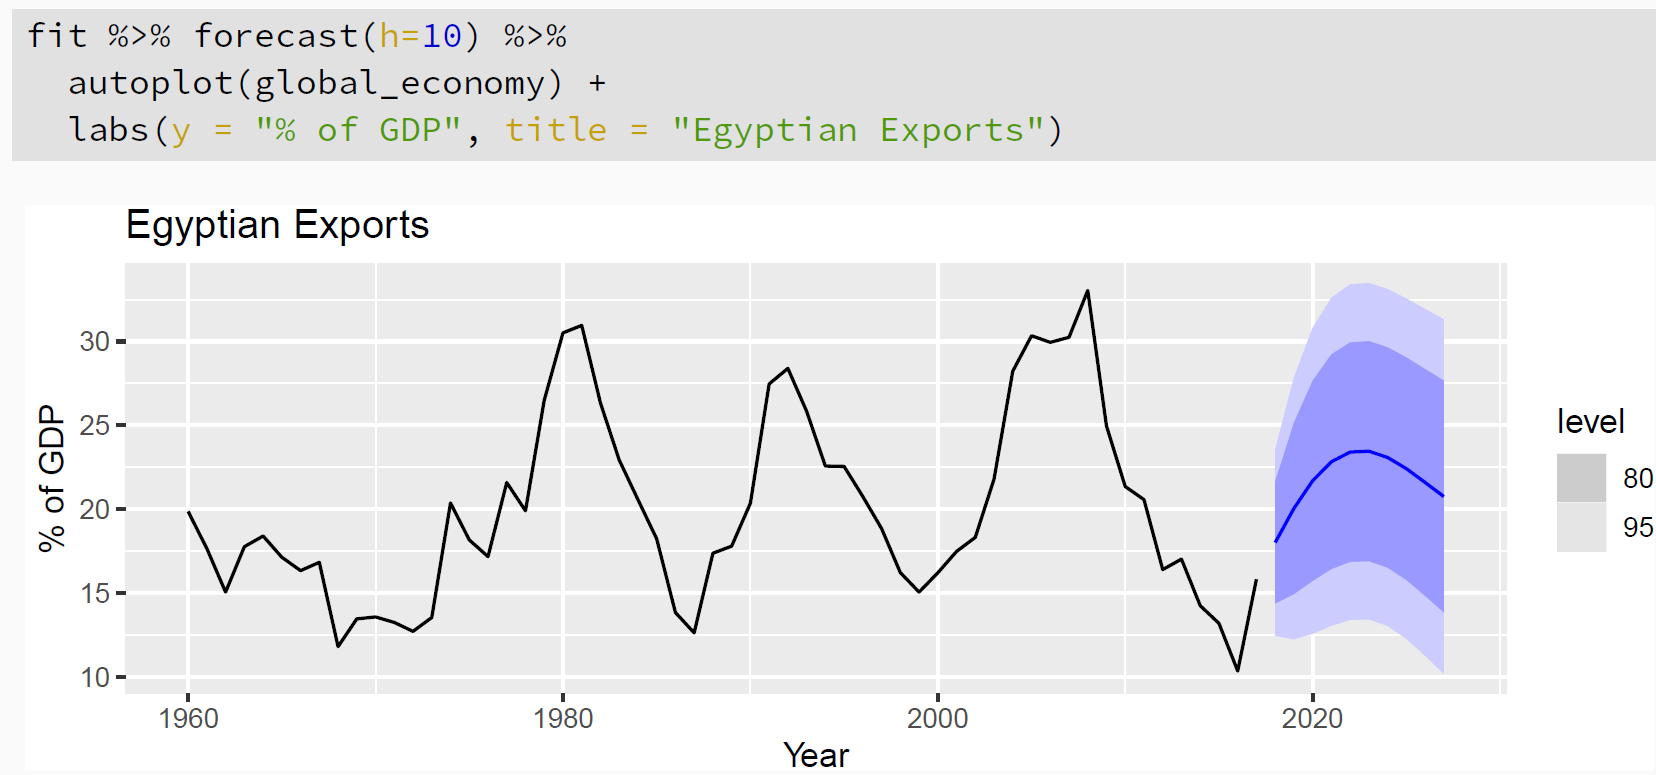
\includegraphics[width=0.95\paperwidth]{../static/course_2_img/egyptian_exports_forecasts.PNG}}     
\end{frame}


\subsection{Modelling and Forecasting with ARIMA Models}


\begin{frame}
  \frametitle{General Approach}
  \begin{itemize}
  \item \textbf{Plot the data}. Identify any unusual observations
  \item If necessary, \textbf{transform the data} (using a Box-Cox transformation) to stabilize the variance
  \item If the data are non-stationary, \textbf{first-difference} it until stationarity
  \item \textbf{Examine the ACF/PACF}: is an $AR(p)$ or $MA(q)$ reasonable assumptions
  \item Try your chosen models: use AIC to compare with other models
  \item Plot the residuals, look at the residuals ACF. Residuals should look like a \textbf{white noise}.
  \item Once the residuals look like a white noise, \textbf{compute the forecasts}    
  \end{itemize}
\end{frame}


\begin{frame}
  \frametitle{Parameters Selection: Algorithm}
  \begin{block}{ARIMA Specification}
    \begin{equation*}
    \phi(B) (1-B)^d y_t = c + \theta(B) \epsilon_t      
    \end{equation*}

    \begin{wideitemize}
      \item Need the select the appropriate order for $p, q, d$
    \end{wideitemize}
    
  \end{block}

\medskip
  
\textbf{Hyndman and Khandasar (2008) selection algorithm}:\\

\begin{wideitemize}
  \item Select the differencing order (=number of differences) \textbf{$d$} and \textbf{$D$} using KPSS test
  \item Select $p, q$ by minimizing AICs
  \item Use stepwise search to traverse model space (= test different combinations of $p, q$ for robustness)
\end{wideitemize}

\end{frame}


\begin{frame}
  \frametitle{Selection Algorithm}
  \begin{alertblock}{Aikaike Information Criteria (AIC)}
    \begin{equation*}
      AIC = -2 \text{log}(L) + 2(p+q+k+1) \left[ 1 + \frac{(p+q+k+2)}{T-p-q-k-2} \right]
    \end{equation*}
    \begin{itemize}
    \item where $L$ is the maximized likelihood fitted to the \emph{differenced data}
    \item Degree of freedom: if the model embedds a constant $c$, $k=1$, else $k=0$
    \end{itemize}    
  \end{alertblock}

  Steps:\\

  \begin{wideenumerate}
  \item Select the current model, with the smallest AIC from the most parcimonious
    \begin{itemize}
    \item ARIMA(0,d, 0), ARIMA(1, d, 0), ARIMA(0, d, 1), ARIMA(1, d, 1) and ARIMA(2, d, 2)
    \end{itemize}
  \item Consider \textbf{variations} of the current model:
    \begin{itemize}
    \item Vary one of $p, q$ from current model by $\pm 1$
    \item $p, q$ both vary from current model by $\pm 1$
    \item Include/exclude the constant $c$ from the current model
    \end{itemize}
  \item The model with the lowest $AIC$ becomes the current model. Repeat step 2 until no lowest AIC can be found (traverse model space)
  \end{wideenumerate}

  
\end{frame}

\begin{frame} 
  \frametitle{ARIMA Selection}
  \makebox[\linewidth]{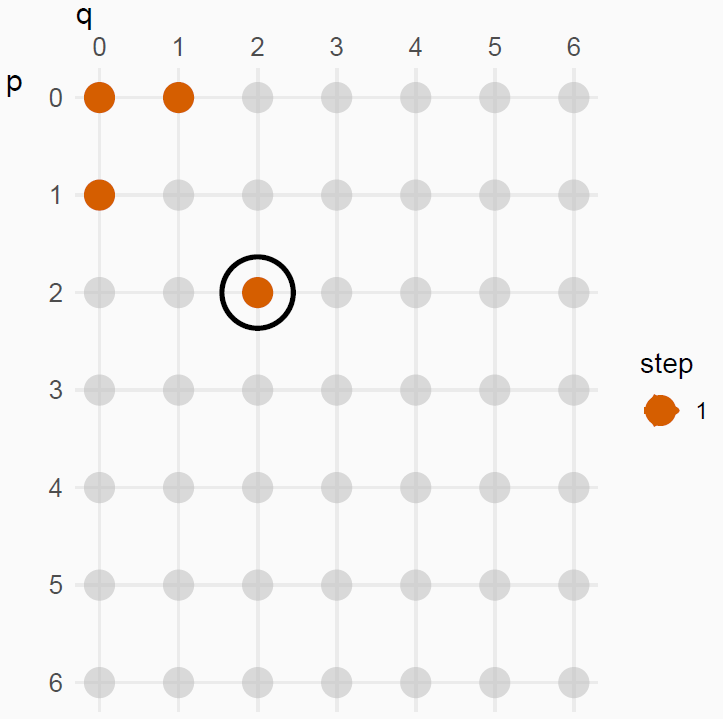
\includegraphics[height=0.95\paperheight]{../static/course_2_img/arima_selection_1.PNG}}     
\end{frame}


\begin{frame} 
  \frametitle{ARIMA Selection}
  \makebox[\linewidth]{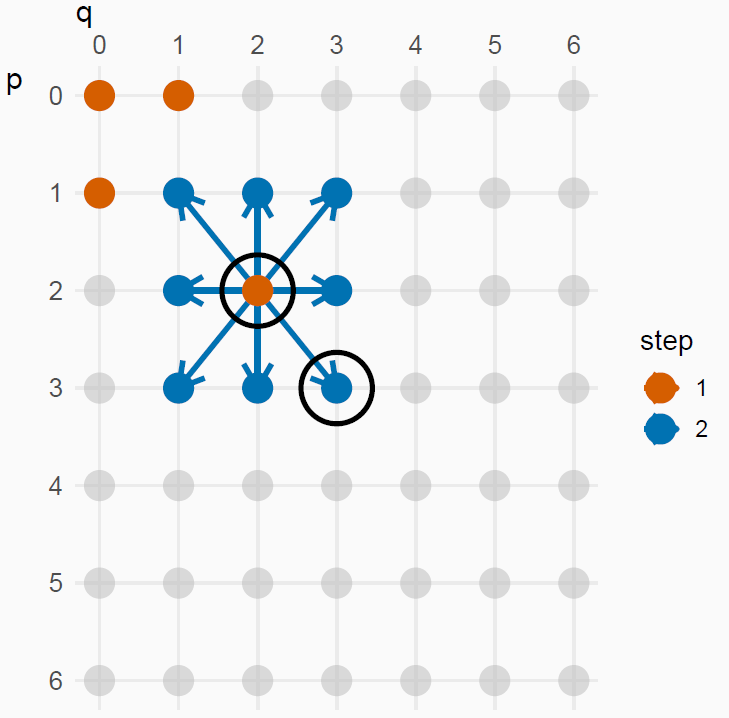
\includegraphics[height=0.95\paperheight]{../static/course_2_img/arima_selection_2.PNG}}     
\end{frame}


\begin{frame} 
  \frametitle{ARIMA Selection}
  \makebox[\linewidth]{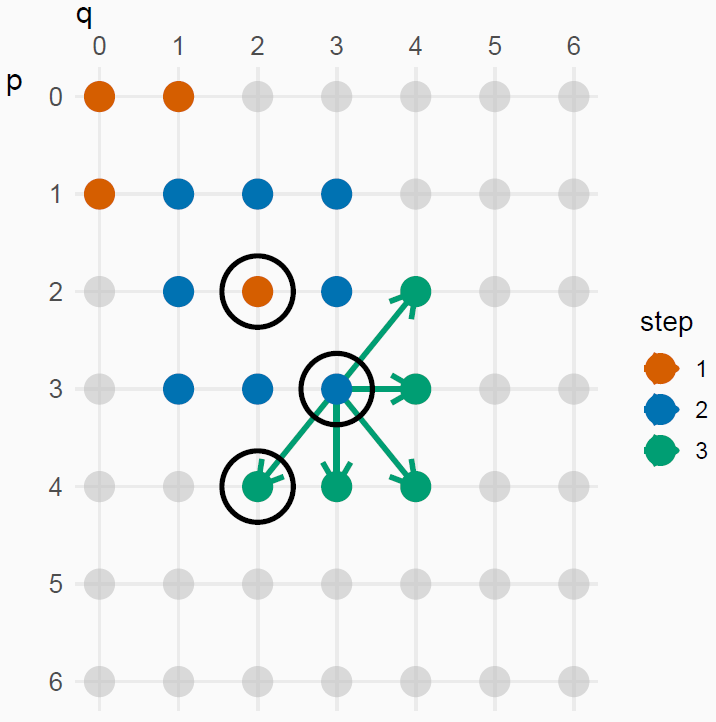
\includegraphics[height=0.95\paperheight]{../static/course_2_img/arima_selection_3.PNG}}     
\end{frame}

\begin{frame} 
  \frametitle{ARIMA Selection}
  \makebox[\linewidth]{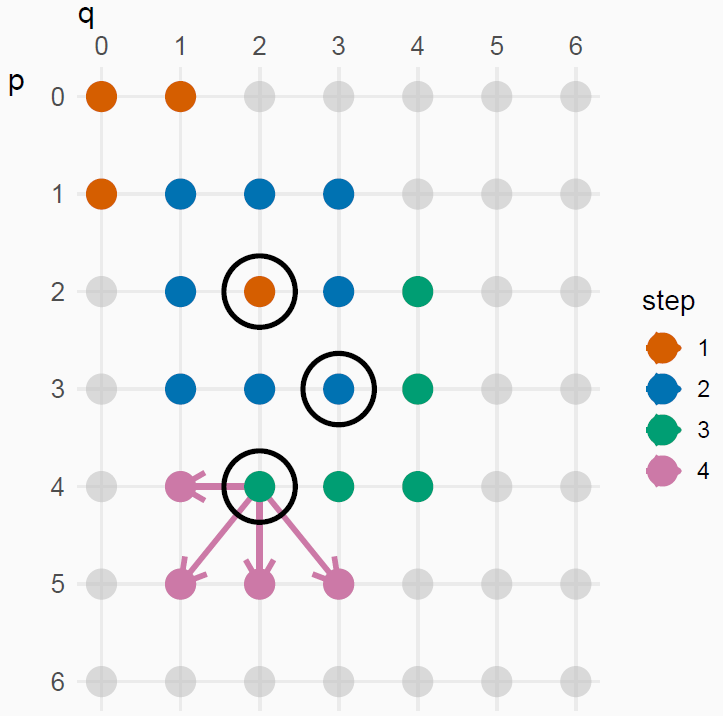
\includegraphics[height=0.95\paperheight]{../static/course_2_img/arima_selection_4.PNG}}     
\end{frame}




\begin{frame} % Need to be redone
  \frametitle{Modelling Process}
  \makebox[\linewidth]{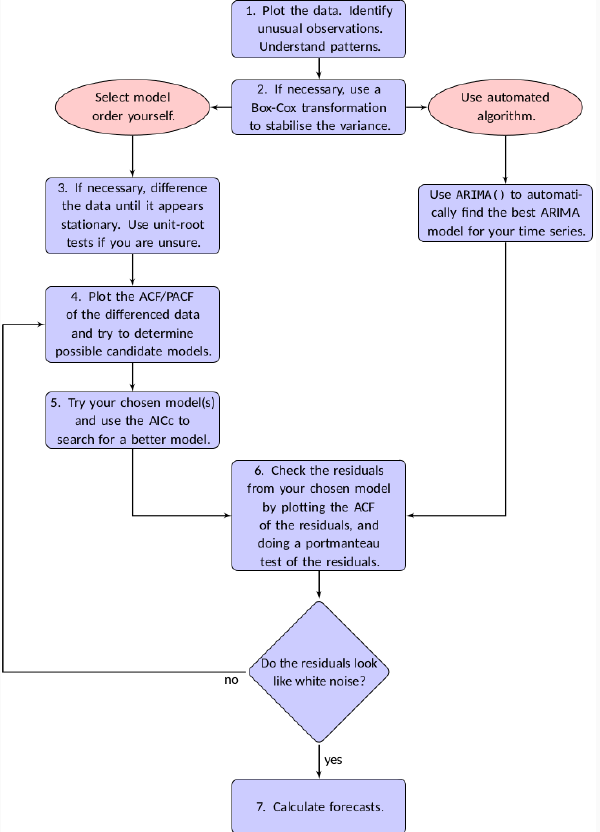
\includegraphics[height=0.95\paperheight]{../static/course_2_img/model_process.PNG}}     
\end{frame}



\begin{frame}
  \frametitle{Point Forecasts}

  General approach:\\
  \medskip

  \begin{wideitemize}
    \item Rearrange the ARIMA equation so that $y_t$ is on the left-hand side
    \item Convert from polynomial backshift to companion form
    \item On the right hand-side, replace the future observations by their forecasts, the future errors by zeros, and the past errors by the corresponding residuals
    \item Start with $h=1$; iterate with $h=2, 3, \dots$
  \end{wideitemize}
  
\end{frame}


\begin{frame}
  \frametitle{Example with an ARIMA(3, 1, 1): Rearrangements}

  \begin{block}{Specification}
    \begin{equation*}
      \underbrace{(1 - \phi_1B - \phi_2B^2 - \phi_3B^3)}_{AR(3)}\underbrace{(1-B)}_{I(1)}y_t = \underbrace{(1+\theta_1 B)\epsilon_t}_{MA(1)}
    \end{equation*}
  \end{block}
  
    \begin{itemize}
    \item Distribute the backshift:
      \begin{equation*}
      \left[1 - (1+\phi_1) B + (\phi_1 - \phi_2) B^2 + (\phi_2-\phi_3) B^3 + \phi_3 B^4 \right] y_t = (1+\theta_1 B)\epsilon_t  
      \end{equation*}
      
    \item Express as a function of $y_t$:
      \begin{equation*}
      y_t - (1+\phi_1)y_{t-1} + (\phi_1 - \phi_2)y_{t-2} + (\phi_2 - \phi_3)y_{t-3} + \phi_3 y_{t-4} = \epsilon_t + \theta_1 \epsilon_{t-1}  
      \end{equation*}
    
    \item Rearrange:
      \begin{equation*}
y_t = (1+\phi_1)y_{t-1} - (\phi_1 - \phi_2)y_{t-2} - (\phi_2 - \phi_3)y_{t-3} - \phi_3 y_{t-4} + \epsilon_t + \theta_1 \epsilon_{t-1}        
      \end{equation*}
      
    \end{itemize}  
\end{frame}


\begin{frame}
  \frametitle{Example with an ARIMA(3, 1, 1): Iterative Replacement}

  \begin{block}{Component Form}
    \begin{equation*}
      y_t = (1+\phi_1)y_{t-1} - (\phi_1 - \phi_2)y_{t-2} - (\phi_2 - \phi_3)y_{t-3} - \phi_3 y_{t-4} + \epsilon_t + \theta_1 \epsilon_{t-1}
    \end{equation*}
  \end{block}
  
  \begin{wideenumerate}
  \item Start at a given $T$, known. Plug $T$ in the formula to obtain the expression of $T+1$
    \begin{equation*}
      y_{T+1} = (1+\phi_1)y_{T} - (\phi_1 - \phi_2)y_{T-1} - (\phi_2 - \phi_3)y_{T-2} - \phi_3 y_{T-3} + \epsilon_{T+1} + \theta_1 \epsilon_{T}
    \end{equation*}

  \item Problem: $\epsilon_{T+1}$ is unknown. Put it at 0 and replace $\epsilon_{T}$ by the fitted residuals $\hat{\epsilon_{T}}$
    \begin{equation*}
      y_{T+1} = (1+\phi_1)y_{T} - (\phi_1 - \phi_2)y_{T-1} - (\phi_2 - \phi_3)y_{T-2} - \phi_3 y_{T-3} +  \theta_1 \hat{\epsilon_{T}}
    \end{equation*}

\item Likewise, iterate for next periods, $T+2, T+3, etc.$
    
    \end{wideenumerate}  
\end{frame}


\begin{frame}
  \frametitle{Prediction Intervals}


  \begin{block}{95\% Prediction Interval}
    \begin{equation*}
      \hat{y}_{T+h|T} \ \pm \ 1.96\sqrt{v_{T+h|T}}
    \end{equation*}
  \end{block}

    \begin{wideitemize}
    \item $v_{T+1|T} \ = \ \hat{\sigma}^2$ for all ARIMA models, regardless of parameters and orders
      \item Multi-step prediction interval for $ARIMA(0,0,q)$:
      \begin{itemize}
      \item $y_t \ = \ \epsilon_t + \sum_{i=1}^q \theta_i \epsilon_{t-i}$
      \item $V_{T|T+h} \ = \ \hat{\sigma}^2 \left[ \sum_{i=1}^{h-1}\theta_i^2 \right] \qquad \forall \ h = 2, 3, \dots$
      \end{itemize}
      
    \end{wideitemize}      
\end{frame}


\begin{frame}
  \frametitle{Properties of Prediction Intervals}
  \begin{wideenumerate}
    \item Prediction intervals increase in size with the forecasting horizon
    \item Prediction intervals can be difficult to calculate by hand
    \item Calculations assume that the residuals are \textbf{uncorrelated} and \textbf{normally distributed}
    \item Prediction intervals tend to be too narrow compared to the true uncertainty:
      \begin{itemize}
      \item The uncertainty in the parameter estimates has not been accounted for
      \item The ARIMA model assumes that the recent historical patterns won't change during the forecast period
      \item The ARIMA model assumes uncorrelated future errors
      \end{itemize}
  \end{wideenumerate}
\end{frame}

\section{Seasonal ARIMA (SARIMA)}


\begin{frame}
  \frametitle{Non-Stationarity and Seasonal Patterns}
  \makebox[\linewidth]{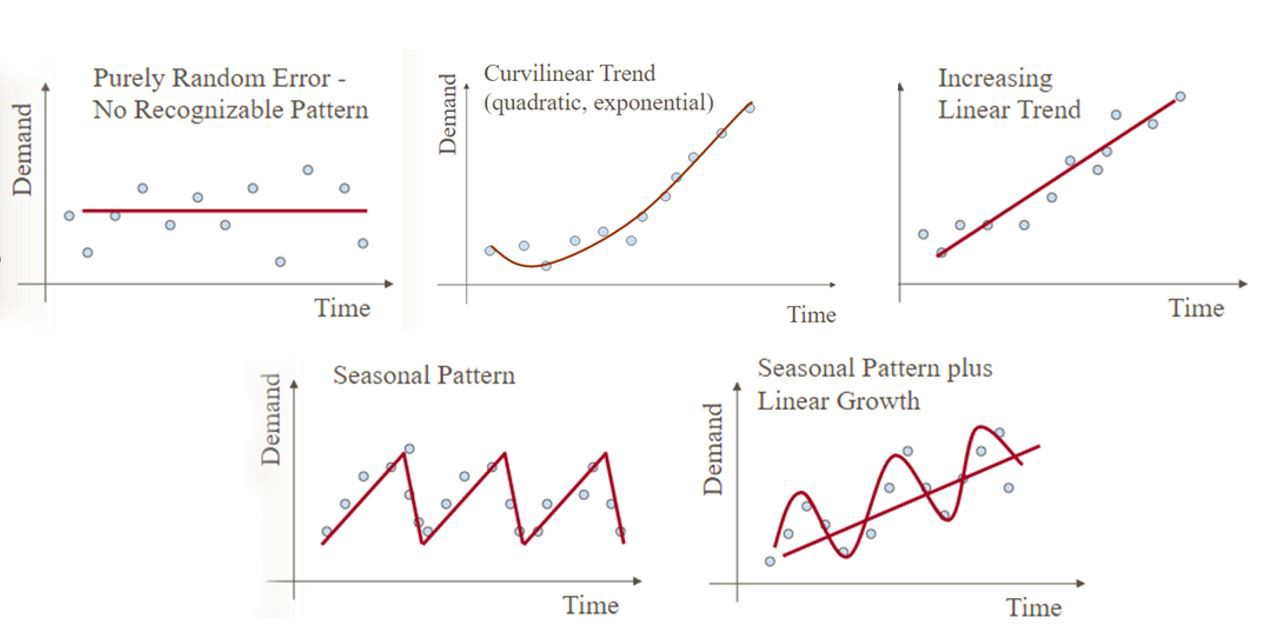
\includegraphics[width=0.75\paperwidth]{../static/course_2_img/time_series_seasonal_patterns.jpeg}}
  \hspace*{15pt}\hbox{\scriptsize Credit:\thinspace{\scriptsize\itshape medium.com}}
\end{frame}


\begin{frame}
  \frametitle{Seasonal ARIMA (SARIMA)}

  \begin{block}{Specification}
    ARIMA  $ \underbrace{(p, d, q)}_{_{\text{Non-Seasonal part of the model}}} \qquad \qquad \underbrace{(P, D, Q)_m}_{\text{Seasonal part of the model}}$
  \end{block}

\medskip
  
where $m$ = number of observations per year
  
\end{frame}


\begin{frame}
  \frametitle{Example: $ARIMA(1,1,1)(1,1,1)_4$}

Example: $ARIMA(1,1,1)(1,1,1)_4$, without constant

\begin{equation*}
  \underbrace{(1-\phi_1B)}_{\text{Non-Seas. AR1}} \underbrace{(1-\Phi_1B^4)}_{\text{Seas. AR1}}\underbrace{(1-B)}_{\text{Seas. Diff.}} \qquad = \qquad \underbrace{(1+\theta_1 B)}_{\text{Non-seas. MA(1)}} \underbrace{(1+\Theta_1 B^4)}_{\text{Seasonal MA(1)}}\epsilon_t
\end{equation*}

\medskip

  All factors can be multiplied out to obtain the model's component form
\end{frame}



\begin{frame}
  \frametitle{US Census Canonical Models}

  The US Census Bureau uses the following models the most often:

  \begin{wideitemize}
  \item $ARIMA(0,1,1)(0,1,1)_m$ with log transformation
  \item $ARIMA(0,1,2)(0,1,1)_m$ with log transformation
  \item $ARIMA(2,1,0)(0,1,1)_m$ with log transformation
  \item $ARIMA(0,2,2)(0,1,1)_m$ with log transformation
  \item $ARIMA(2,1,2)(0,1,1)_m$ with \textbf{no} transformation    
  \end{wideitemize}  
\end{frame}


\begin{frame}
  \frametitle{Intuition}

  The seasonal part of an AR or MA model will be seen in the seasonal lags of the PACF and ACF


  \begin{exampleblock}{$ARIMA(0,0,0)(0,0,1)_{12}$  will show}

    \begin{itemize}
    \item A spike at lag 12 in the ACF but no other significant spikes
    \item The PACF will show exponential decay in the seasonal lags; that is, at lags 12, 24, 36, etc.
    \end{itemize}
    
  \end{exampleblock}
  
\medskip

  \begin{exampleblock}{$ARIMA(0,0,0)(1,0,0)_{12}$  will show}

    \begin{itemize}
    \item Exponential lags in the seasonal lags of the ACF
    \item A single significant spike at lag 12 in the PACF
    \end{itemize}
    
  \end{exampleblock}

\end{frame}


\begin{frame}
  \frametitle{Application:  US Leisure Employment and Hospitality}
     \makebox[\linewidth]{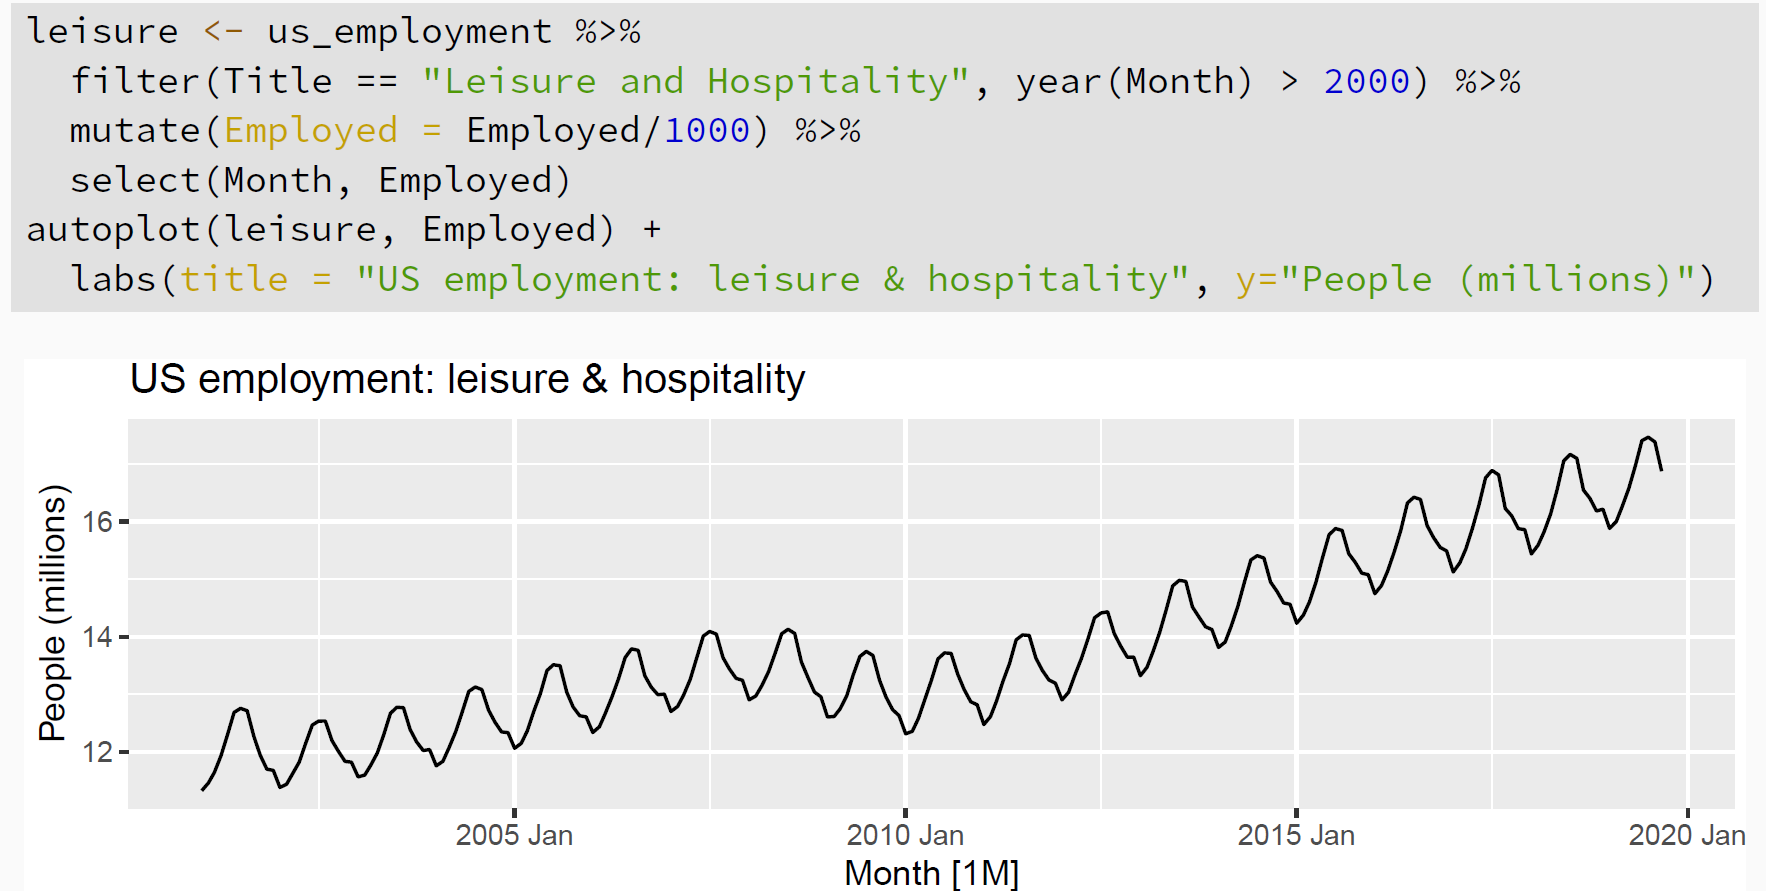
\includegraphics[width=0.95\paperwidth]{../static/course_2_img/us_leisure_1.PNG}}  
\end{frame}

\begin{frame}
  \frametitle{Application:  US Leisure Employment and Hospitality}
     \makebox[\linewidth]{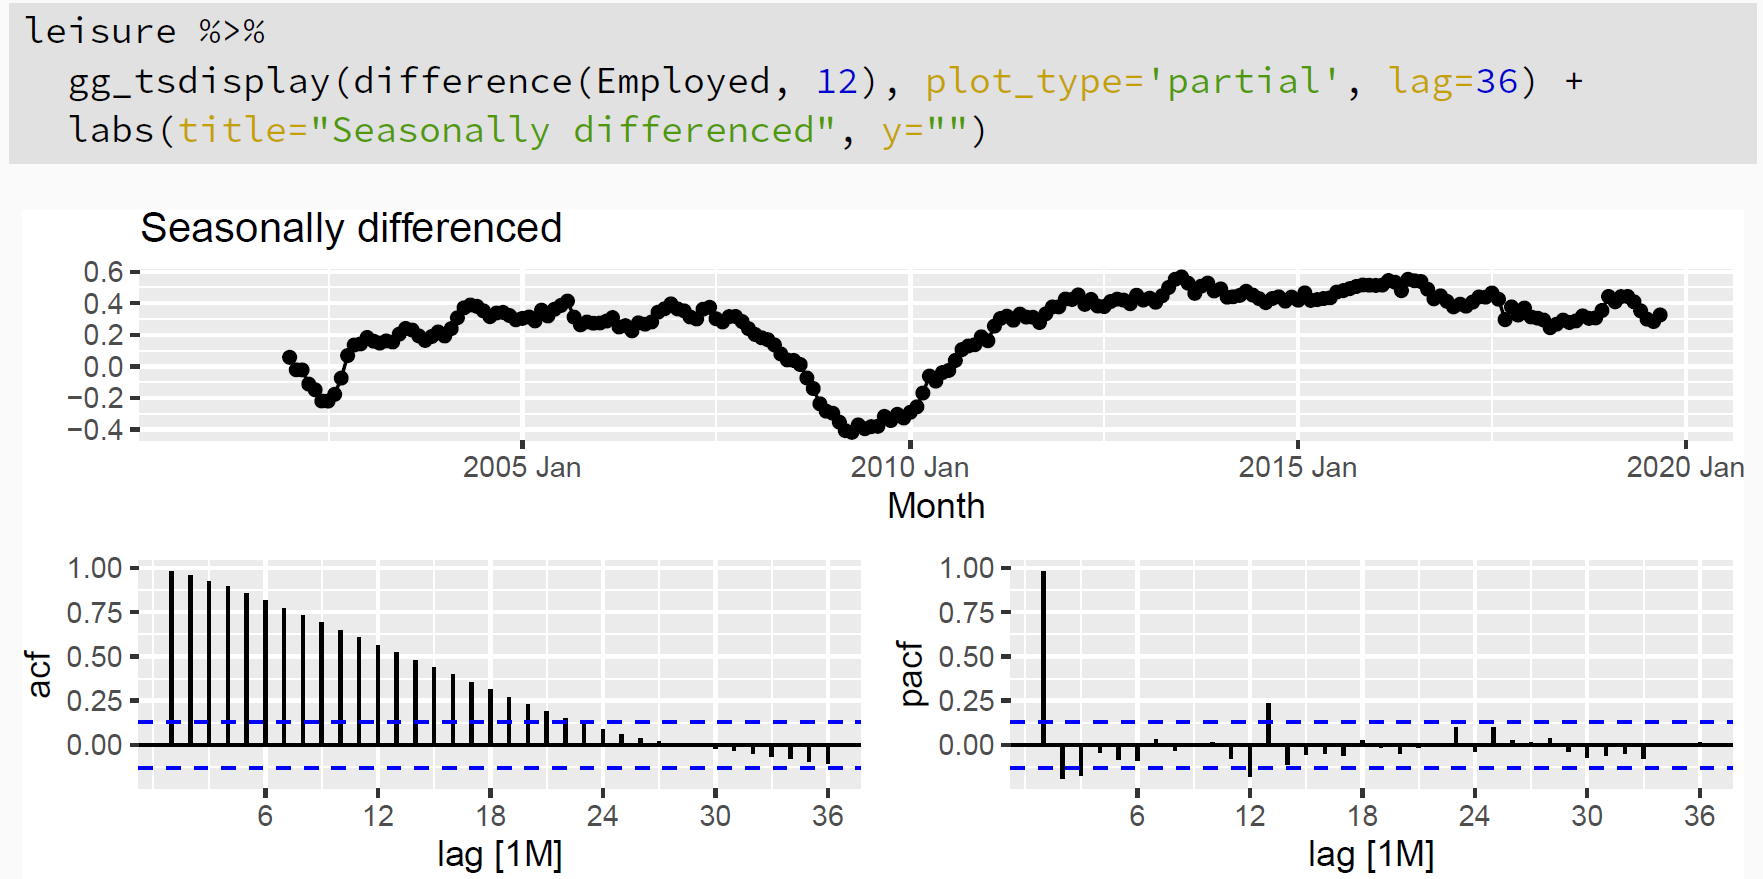
\includegraphics[width=0.95\paperwidth]{../static/course_2_img/us_leisure_2.PNG}}  
\end{frame}


\begin{frame}
  \frametitle{Application:  US Leisure Employment and Hospitality}
     \makebox[\linewidth]{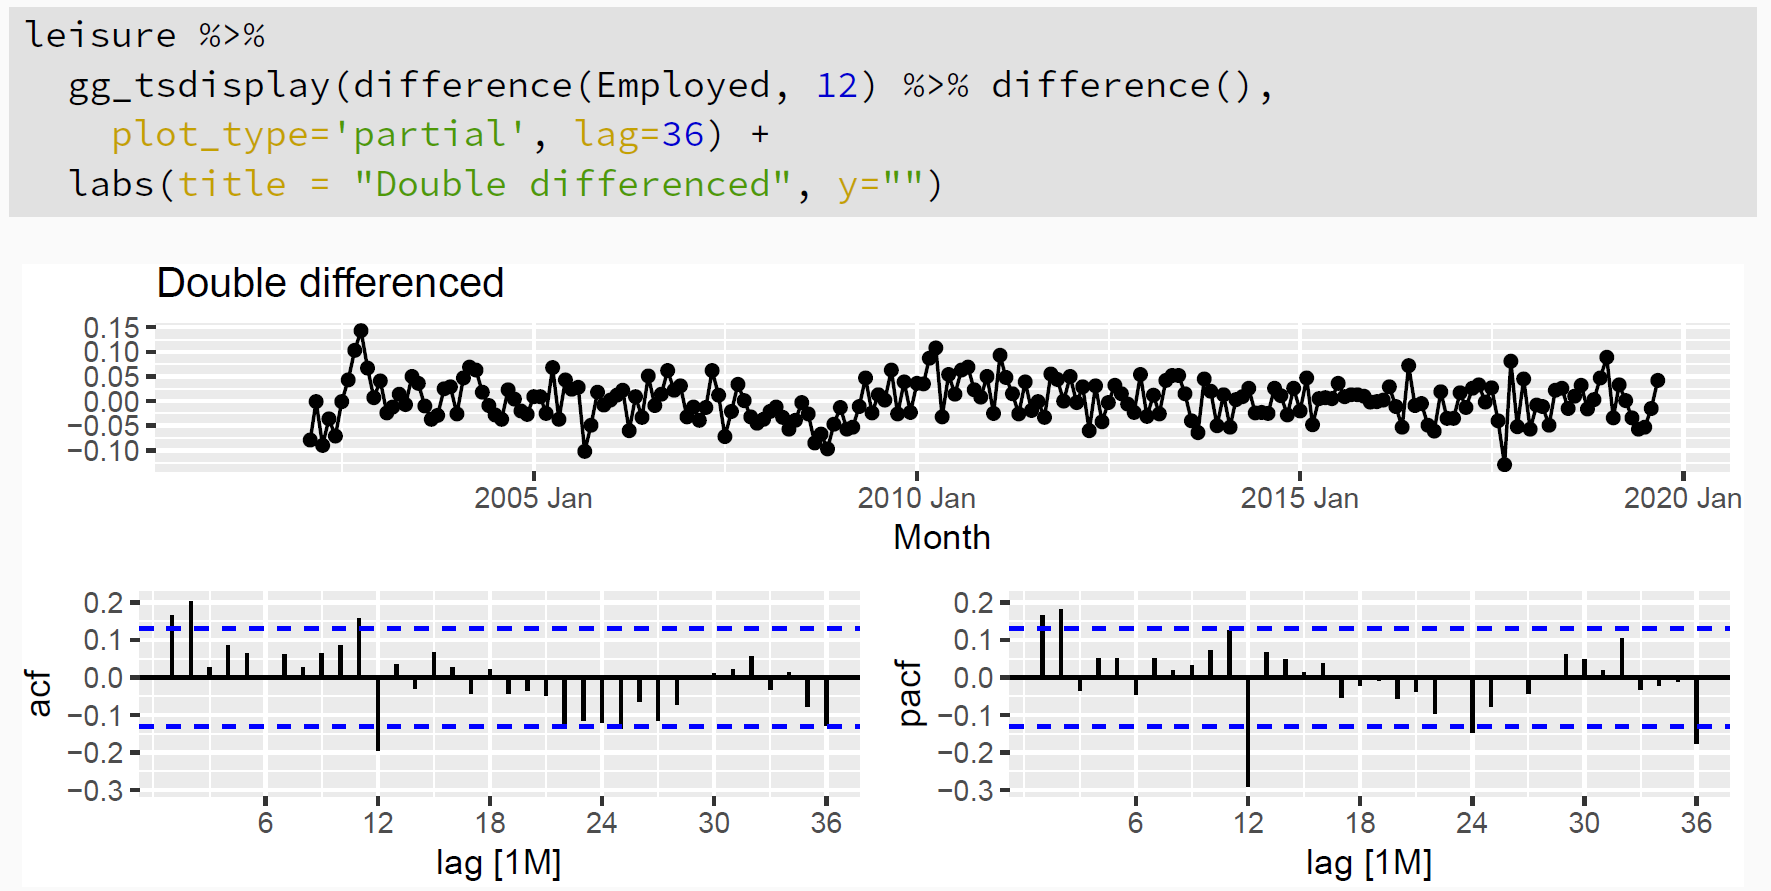
\includegraphics[width=0.95\paperwidth]{../static/course_2_img/us_leisure_3.PNG}}  
\end{frame}

\begin{frame}
  \frametitle{Application:  US Leisure Employment and Hospitality}
     \makebox[\linewidth]{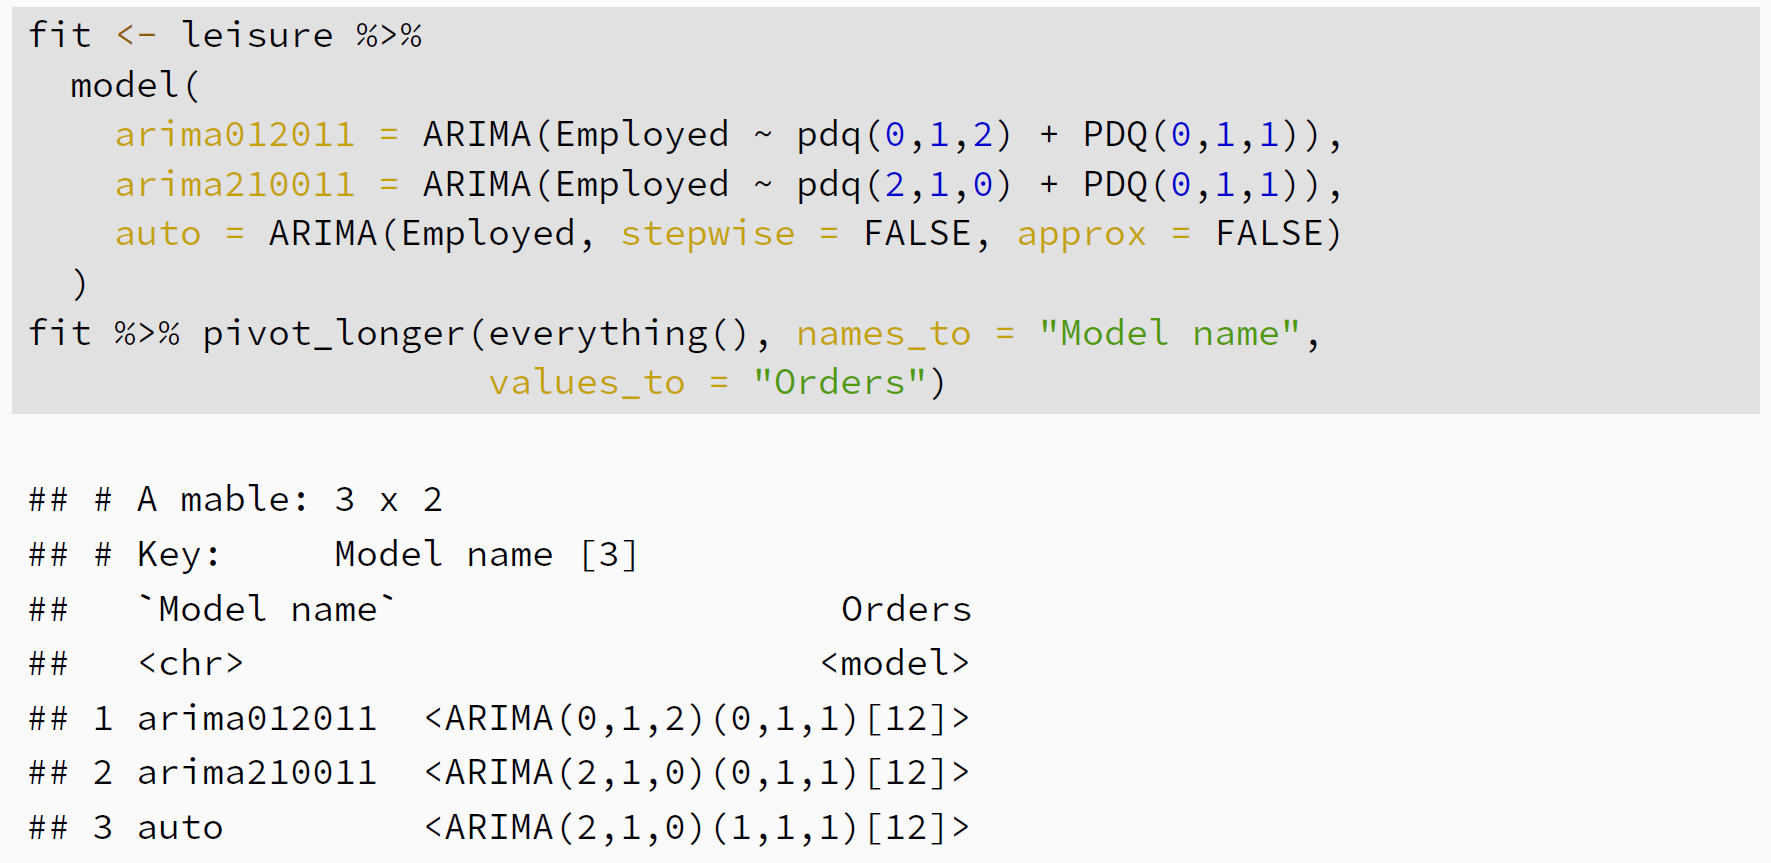
\includegraphics[width=0.95\paperwidth]{../static/course_2_img/us_leisure_4.PNG}}  
\end{frame}


\begin{frame}
  \frametitle{Application:  US Leisure Employment and Hospitality}
     \makebox[\linewidth]{\includegraphics[width=0.95\paperwidth]{../static/course_2_img/us_leisure_5.PNG}}  
\end{frame}



\begin{frame}
  \frametitle{Treatment of Seasonality}

  \begin{wideitemize}
    \item Daily data can exhibit multiple seasonal periodicities. This is a complication for all high-frequency forecasting problems: day in the month, day in the week, etc.
    \item This comes with additional complexity:
      \begin{itemize}
        \item Months has different number of days
        \item Leap years with different number of days
        \item Weeks do not align with daily cycles (the year is not divisible in an exact number of weeks)
        \end{itemize}
      \item Seasonality can be irregular: Ramadan and some other religious festivities for instance
      \item We use two approaches to deal with complex seasonality
        \begin{enumerate}
        \item Trigonometric representation of seasonality
        \item Simplification of seasonal terms
        \end{enumerate}
  \end{wideitemize}
  
\end{frame}


\begin{frame}
  \frametitle{Problems of an ARIMA with Many Binary Variables}

  \begin{wideitemize}
  \item Often, central banks forecast currency in circulation by including a large number of binary variables (“dummies”) to capture different seasonality patterns. This is called \textbf{binary seasonality}

  \item In general, this approach should be discouraged, because:
    \begin{itemize}
    \item Including a large number of variables imply to estimate many more parameters, hence \textbf{adding parametric noise to the model}
    \item Many parameters are not relevant/useful, \textbf{increasing noise/signal ratio}
    \item Reducing the degrees of freedom spurs the \textbf{risk of overfit}
    \end{itemize}
    
  \item We tested a large number of models in different countries, confirming the relatively bad performance of ARIMA with binary seasonality
    
  \end{wideitemize}

\end{frame}



\begin{frame}
  \frametitle{Binary and Trigonometric Seasonality}
  \begin{itemize}
  \item Consider a single deterministic seasonal cycle. We can model this either by:
    \begin{itemize}
      \item \textbf{Indicator variables} (e.g. friday's dummy: equals to 1 on Friday and 0 otherwise)
      \item \textbf{Trigonometric variables} (cf. Fourier Analysis): Trigonometric approach
    \end{itemize}
  \end{itemize}
\makebox[\linewidth]{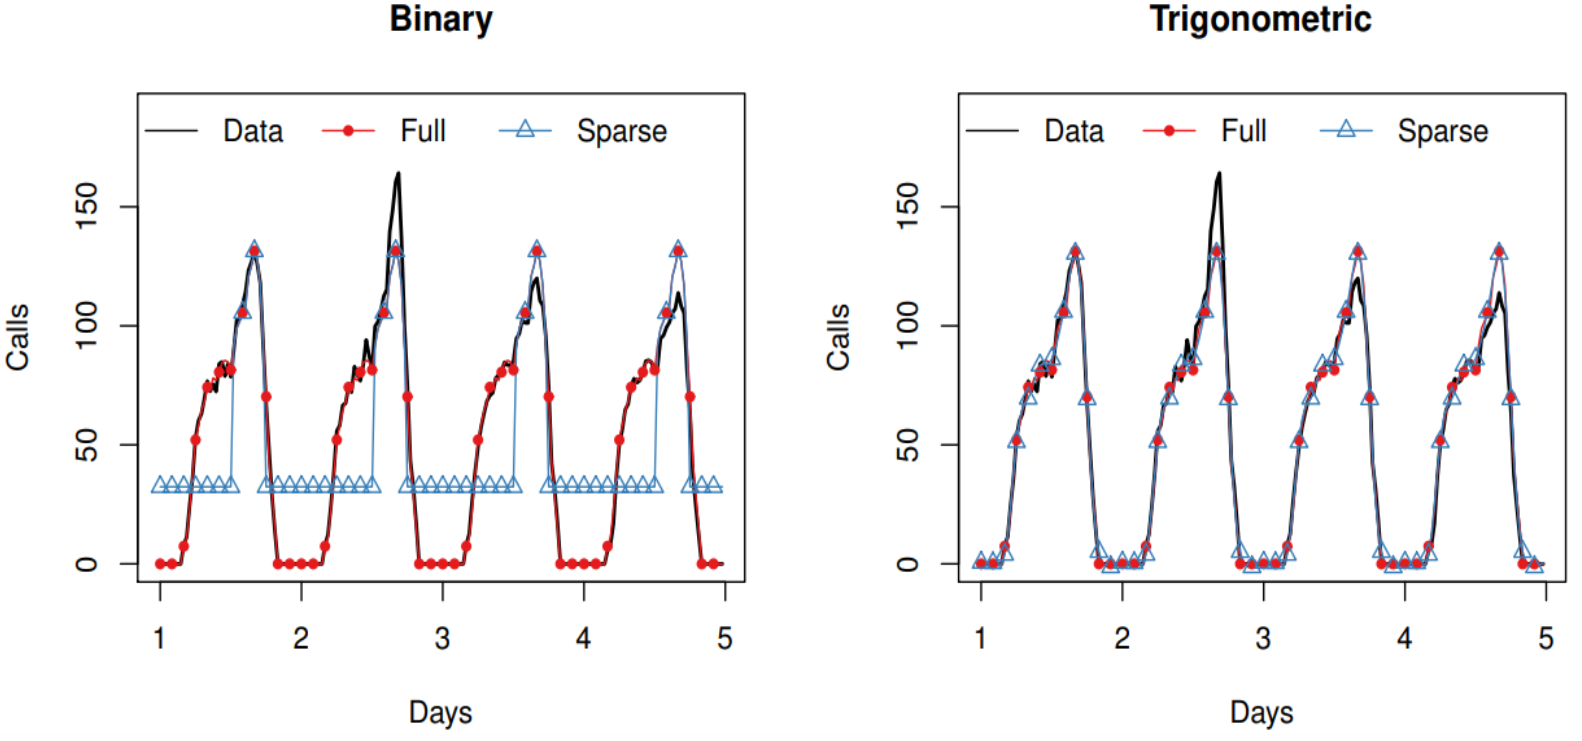
\includegraphics[width=0.65\paperwidth]{../static/course_2_img/binary_trigonometric.PNG}}    
\end{frame}


\begin{frame}
  \frametitle{Binary and Trigonometric Seasonality: Pros and Cons}
  \begin{wideitemize}
  \item Elimination of terms:
    \begin{itemize}
    \item Eliminating terms from the binary (indicator variable) representation, removes the effect of seasonal periods
    \item Eliminating terms in the trigonometric representation results in smoother approximations of the seasonal shape 
    \item Elimination of terms can be done using information criteria
    \end{itemize}
  \item Besides, trigonometric representation is more parsimonious, as it involves less parameters to estimate: reduce parametric noise
  \item Model-wise: ARIMA with dummy variables for seasonality versus SARIMA (“Seasonal ARIMA”) that suggests stochastic seasonality
  \end{wideitemize}
\end{frame}


\begin{frame}
  \frametitle{ARIMA with Trigonometric Seasonality}
  \begin{wideitemize}
    \item $ARIMA(p, d, q)(P_1, D_1, Q_1)_{S_1}$
    \item $S_1 = 5$ days in the week
    \item The model contains trigonometric variables of the form sin$\frac{2 t \times i_j \pi}{S_j}$ and cos$\frac{2 t \times i_j \pi}{S_j}$
      \begin{itemize}
      \item $i_j$
      \end{itemize}
  \end{wideitemize}
\end{frame}


\subsection{ARIMA versus ETS}

\begin{frame}
  \frametitle{ARIMA versus ETS}
  While the general perception sees ARIMA has more general than ETS, this is not exactly true:
  \begin{wideitemize}
  \item Linear ETS are all special cases of ARIMA models
  \item Non-linear exponential smoothing model (e.g. multiplicative) have no ARIMA equivalent
  \item Many ARIMA have no linear exponential smoothing model equivalent
  \item ETS models are non-stationary. The number of roots depends on the inclusion of seasonal terms or not
  \end{wideitemize}
\end{frame}

\begin{frame}
  \frametitle{ARIMA versus ETS Models}
     \makebox[\linewidth]{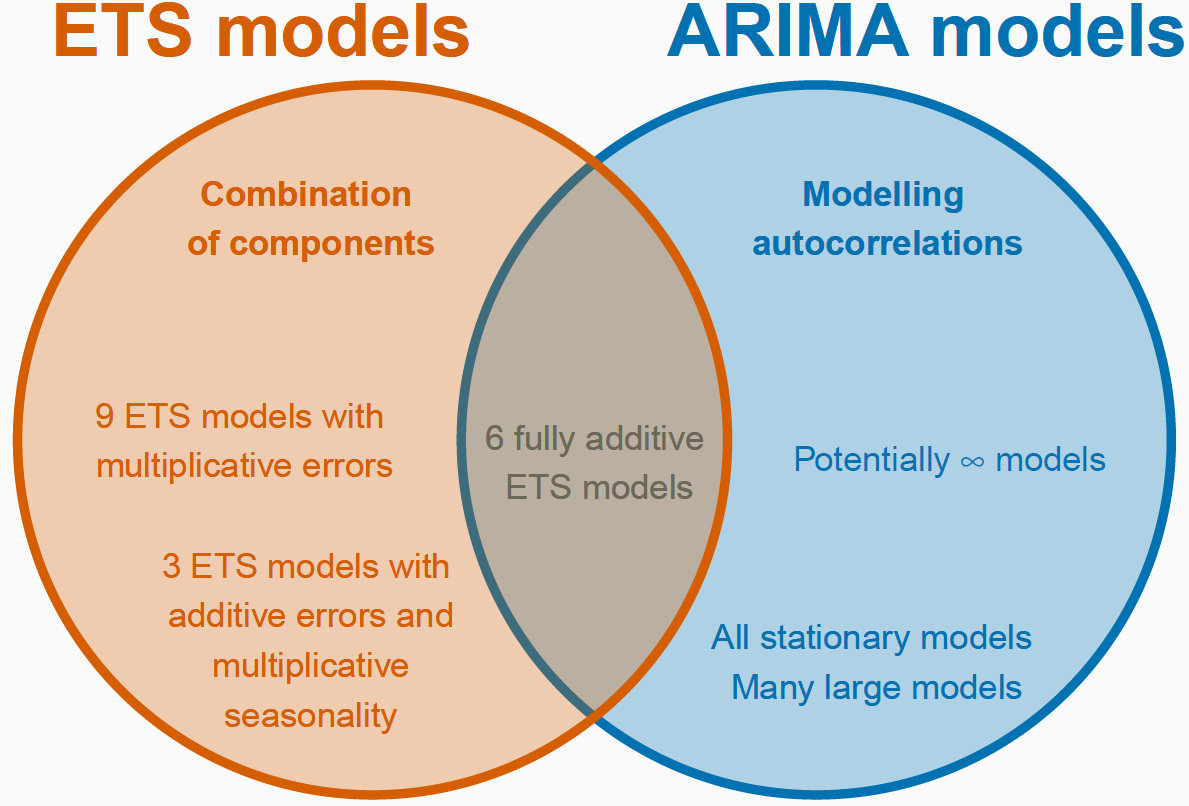
\includegraphics[width=0.7\paperwidth]{../static/course_2_img/ARIMA_vs_ETS.PNG}}  
\end{frame}



\begin{frame}
  \frametitle{Question 1}

\textbf{What are the problems associated with using many binary variables to model seasonality? Multiple answers possible:}\\
\bigskip
\begin{wideenumerate}
  \item Complicated to estimate
  \item Takes excessive computation time 
  \item Add parametric noise
  \item Risk of overfit
\end{wideenumerate}  
\end{frame}

\section{Advanced Seasonal Models}

\begin{frame}
 \frametitle{Bias Identification}
  \makebox[\linewidth]{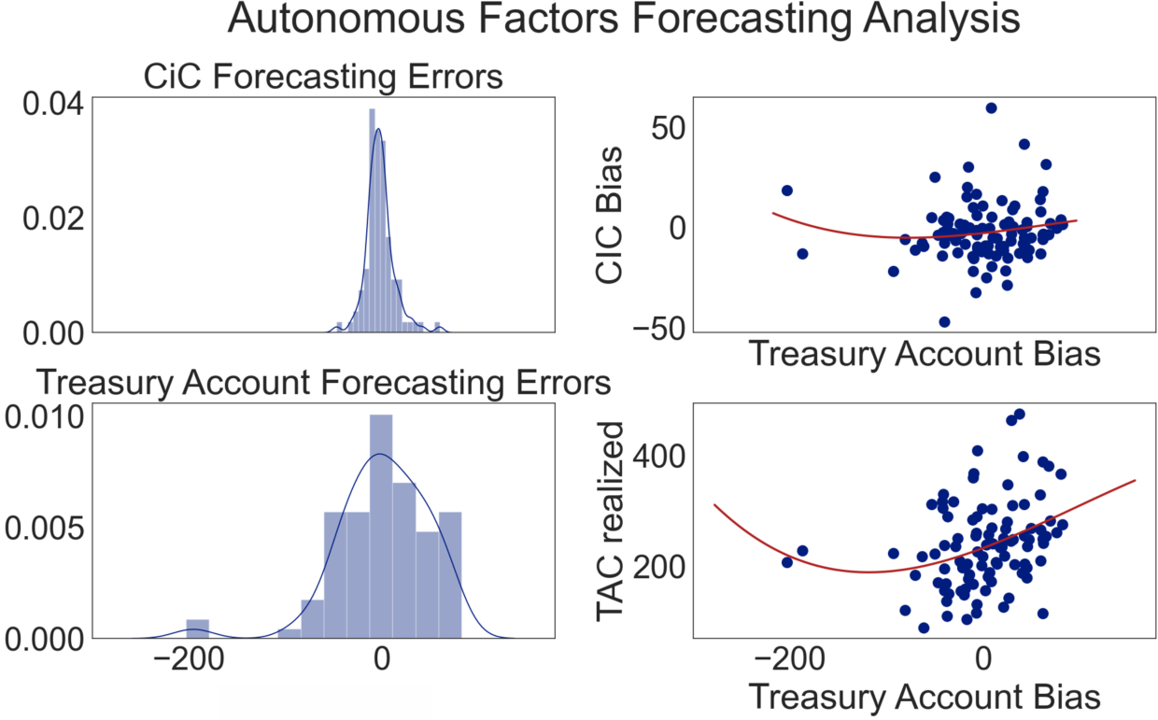
\includegraphics[width=0.85\paperwidth]{../static/course_3_img/bias_correction.png}}
 \hspace*{15pt}\hbox{\scriptsize Credit:\thinspace{\scriptsize\itshape Author}}      
 \end{frame}


  \begin{frame}
    \frametitle{Advanced Models Typology}

  \begin{wideitemize}
    \item \textbf{ETS with trigonometric} multiple seasonalities and indicators for events
    \item \textbf{ARIMA with trigonometric} multiple seasonalities and indicators for events
    \item \textbf{ARIMA with stochastic} multiple seasonalities and indicators for events
    \item \textbf{TBATS} – a state space model with exponential smoothing, stochastic trigonometric patterns, Cox-Box transformation and ARIMA errors. TBATS cannot incorporate events 
    \item \textbf{Composite TBATS} – where the local level and events are modelled with ETS and the seasonality/trend with TBATS
    \end{wideitemize}
    
  \end{frame}
  

    \begin{frame}
      \frametitle{Box Cox Transformation}

      \begin{wideitemize}
        \item The Box-Cox transformation is used to transform non-Gaussian data $y_t$ into Gaussian  data
        \item Working with Gaussian data makes it easier to apply the standard model in econometrics
        \item The Box Cox transformation works with a parameters $\lambda$ that takes values between $[-5, 5]$

        \item For positive $y_t$ data:
          \begin{itemize}
          \item $y(\lambda) = \frac{y^{\lambda}-1}{\lambda}$ if $\lambda neq 0$
          \item $\text{log}(y)$ if $\lambda = 0$
          \end{itemize}

        \item For negative $y_t$ data, use an extra parameter $\lambda_2$ 
          \begin{itemize}
          \item $y(\lambda) = \frac{(y + \lambda_2)^{\lambda}-1}{\lambda}$ if $\lambda neq 0$
          \item $\text{log}(y + \lambda_2)$ if $\lambda = 0$
          \end{itemize}          
      \end{wideitemize}      
    \end{frame}


    \begin{frame}
      \frametitle{Transforming Data with the Box Cox Transformation}
  \makebox[\linewidth]{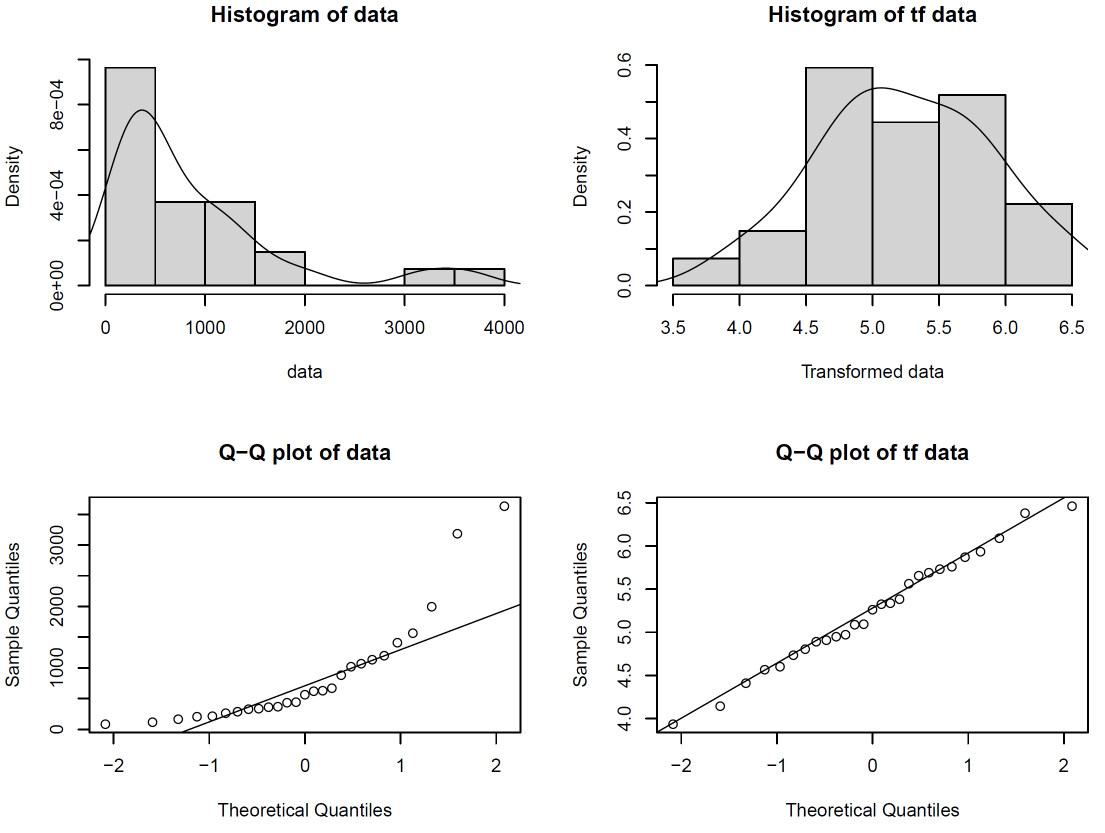
\includegraphics[width=0.75\paperwidth]{../static/course_3_img/box_cox_data_transformation.PNG}}
  \hspace*{15pt}\hbox{\scriptsize Credit:\thinspace{\scriptsize\itshape https://universeofdatascience.com/}}      
    \end{frame}

    \begin{frame}
      \frametitle{The TBATS Model: Overview}
  \makebox[\linewidth]{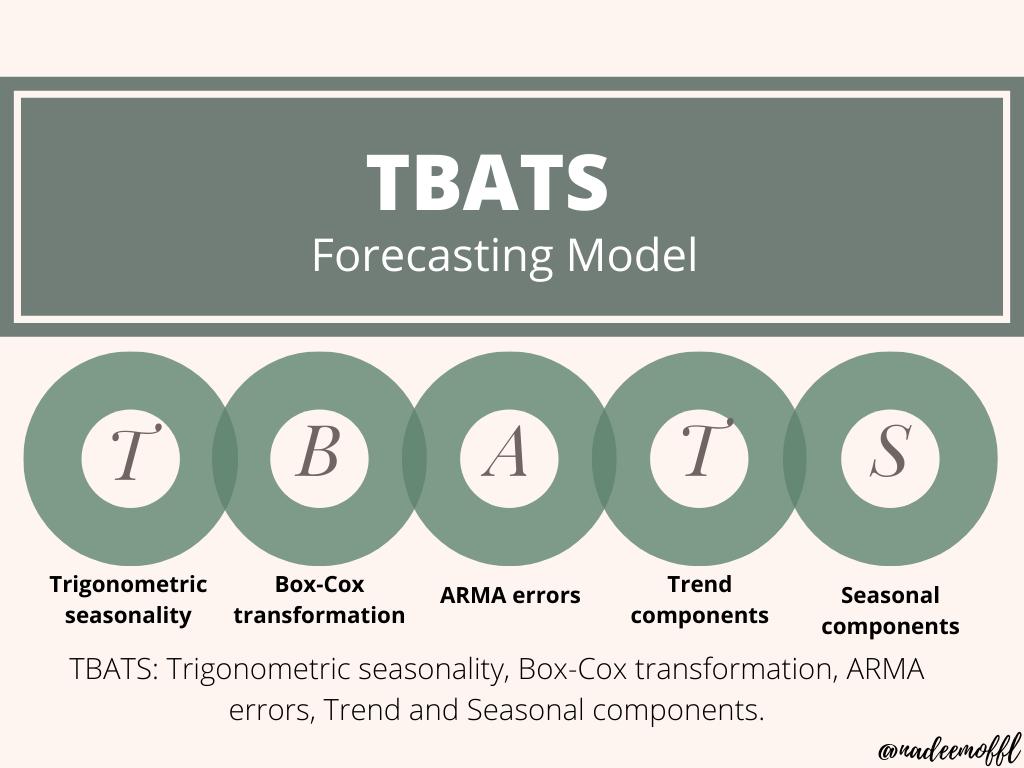
\includegraphics[width=0.75\paperwidth]{../static/course_3_img/TBATS presentation.png}}
  \hspace*{15pt}\hbox{\scriptsize Credit:\thinspace{\scriptsize\itshape https://medium.com/analytics-vidhya/}}      
    \end{frame}

    
  \begin{frame}
    \frametitle{The TBATS Model: Overview}

    \begin{wideitemize}
    \item Combines in a \textbf{single state-space} model:

      \begin{itemize}
      \item Trigonometric terms to account for seasonality
      \item Box-Cox transformation to account for non-normality and heterogeneity
      \item ARIMA errors to model the residuals short-term dynamic
      \item Trend (potentially damped)        
      \item Seasonal (including multiple and non-integer period)
      \end{itemize}

    \item Main specifications:
      \begin{itemize}
      \item Handles non-integer seasonality, multiple seasonal periods
      \item Entirely automated
      \item Predictions interval often wide
      \item Very slow on long series
      \end{itemize}      
    \end{wideitemize}
    \end{frame}

    
    \begin{frame}
      \frametitle{The TBATS Model: Specification}
  \makebox[\linewidth]{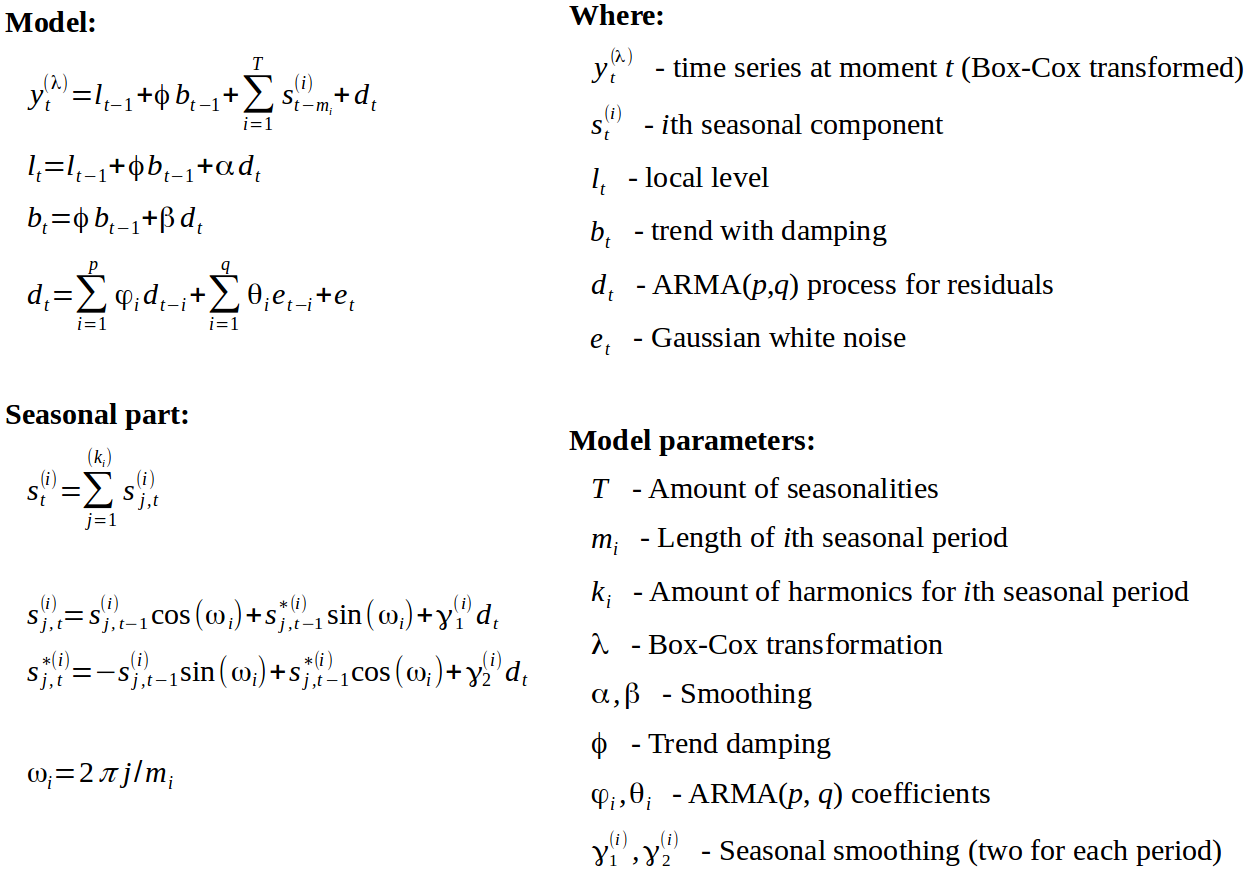
\includegraphics[width=0.75\paperwidth]{../static/course_3_img/TBATS_specification.png}}
  %\hspace*{15pt}\hbox{\scriptsize Credit:\thinspace{\scriptsize\itshape Author}}      
    \end{frame}

    \begin{frame}
      \frametitle{The TBATS Model: Decomposition}
  \makebox[\linewidth]{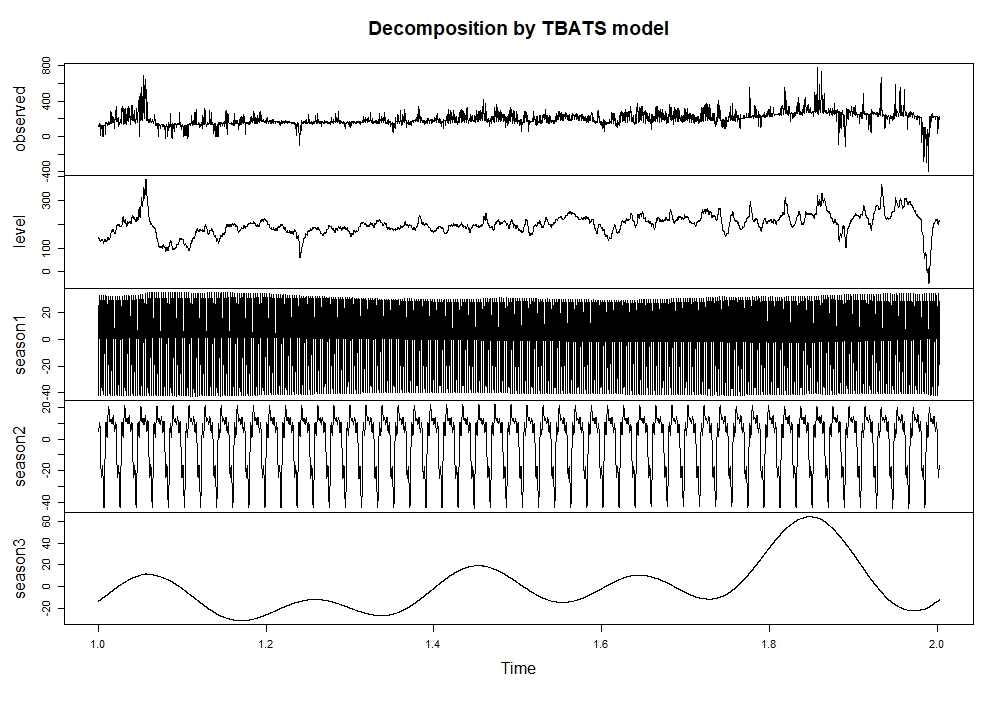
\includegraphics[width=0.75\paperwidth]{../static/course_3_img/TBATS_decomposition.jpg}}
  %\hspace*{15pt}\hbox{\scriptsize Credit:\thinspace{\scriptsize\itshape Author}}      
    \end{frame}




\end{document}